% ****** Start of file apssamp.tex ******
%
%   This file is part of the APS files in the REVTeX 4.2 distribution.
%   Version 4.2a of REVTeX, December 2014
%
%   Copyright (c) 2014 The American Physical Society.
%
%   See the REVTeX 4 README file for restrictions and more information.
%
% TeX'ing this file requires that you have AMS-LaTeX 2.0 installed
% as well as the rest of the prerequisites for REVTeX 4.2
%
% See the REVTeX 4 README file
% It also requires running BibTeX. The commands are as follows:
%
%  1)  latex apssamp.tex
%  2)  bibtex apssamp
%  3)  latex apssamp.tex
%  4)  latex apssamp.tex
%
\documentclass[%
reprint, %% for final paper
superscriptaddress,
%groupedaddress,
%unsortedaddress,
%runinaddress,
%frontmatterverbose, 
%preprint, %% for single-column, double-spacing
%preprintnumbers,
%nofootinbib,
%nobibnotes,
%bibnotes,
 amsmath,amssymb,
 aps,
%pra,
%prb,
%rmp,
%prstab,
%prstper,
%floatfix,
]{revtex4-2}
\usepackage[utf8]{inputenc}
\usepackage{graphicx}% Include figure files
\usepackage{dcolumn}% Align table columns on decimal point
\usepackage{bm}% bold math
\usepackage{hyperref}% add hypertext capabilities
\usepackage[mathlines]{lineno}% Enable numbering of text and display math
\usepackage{amsmath} %for multiline in equation
%\usepackage{comment}

%\linenumbers %for preprint
\relax % Commence numbering lines
%\usepackage[showframe,%Uncomment any one of the following lines to test 
%%scale=0.7, marginratio={1:1, 2:3}, ignoreall,% default settings
%%text={7in,10in},centering,
%%margin=1.5in,
%%total={6.5in,8.75in}, top=1.2in, left=0.9in, includefoot,
%%height=10in,a5paper,hmargin={3cm,0.8in},
%]{geometry}

%abbreviation
\newcommand{\gagg}{\ensuremath{\left|g_{a\gamma\gamma}\right|}}
\newcommand{\ggamma}{\ensuremath{\left|g_{\gamma}\right|}}
\newcommand{\bgagg}{\ensuremath{g_{a\gamma\gamma}}}
\newcommand{\bggamma}{\ensuremath{g_{\gamma}}}
\newcommand{\ma}{\ensuremath{m_a}}
%\def\muev{\ensuremath{\mu~\mathrm{eV}}
\newcommand{\tsys}{\ensuremath{T_\text{sys}}}
\newcommand{\ta}{\ensuremath{T_\text{a}}}
%\newcommand{\muevcc}{\ensuremath{\,\mu\text{e\hspace{-.08em}V\hspace{-0.16em}/\hspace{-0.08em}}c^2}}
\newcommand{\muevcc}{\ensuremath{\,\mu\text{e\hspace{-.08em}V}}}
\newcommand{\MeV}{\ensuremath{\,\text{Me\hspace{-.08em}V}}}
\newcommand{\GeV}{\ensuremath{\,\text{Ge\hspace{-.08em}V}}}
\newcommand{\GeVinv}{\ensuremath{\,\text{Ge\hspace{-.08em}V}^{-1}}}
%\newcommand{\flo}{\ensuremath{4.707504}}
%\newcommand{\fhi}{\ensuremath{4.798147}}
\newcommand{\flo}{\ensuremath{4.70750}}
\newcommand{\fhi}{\ensuremath{4.79815}}
%\newcommand{\mlo}{\ensuremath{19.47}}
%\newcommand{\mhi}{\ensuremath{19.84}}
\newcommand{\mlo}{\ensuremath{19.4687}}
\newcommand{\mhi}{\ensuremath{19.8436}}
\newcommand{\avelimit}{\ensuremath{8.2\times 10^{-14}}} %8.19+-0.38
\newcommand{\ADMXavelimit}{\ensuremath{4.9\times 10^{-14}}} 
\newcommand{\lolimit}{\ensuremath{5.3\times 10^{-14}}} 
\newcommand{\hilimit}{\ensuremath{8.9\times 10^{-14}}} 
% exact number of the average limit 7.6965 x 10^-14 
%\newcommand{\noise}{\ensuremath{2.3}}
\newcommand{\noise}{\ensuremath{1.9 - 2.2}}


\begin{document}

\preprint{APS/123-QED}

%\title{First Results from the Taiwan Axion Search Experiment with Haloscope in the \mlo--\mhi\muevcc\ Mass Range}% Force line breaks with \\
\title{Taiwan Axion Search Experiment with Haloscope: CD102 Analysis Details}% Force line breaks with \\
%\thanks{A footnote to the article title}%

%\author{Ann Author}
% \altaffiliation[Also at ]{Physics Department, XYZ University.}%Lines break automatically or can be forced with \\
%\author{Second Author}%
% \email{Second.Author@institution.edu}
%\affiliation{%
% Authors' institution and/or address\\
% This line break forced with \textbackslash\textbackslash
%}%
%Hsin Chang
\author{Hsin~Chang}\affiliation{Department of Physics, National Central University, Taoyuan City 32001, Taiwan}
%Jing-Yang Chang
\author{Jing-Yang~Chang}\affiliation{Department of Physics, National Central University, Taoyuan City 32001, Taiwan} 
%Yi-Chieh Chang
\author{Yi-Chieh~Chang}\affiliation{National Synchrotron Radiation Research Center, Hsinchu 30076, Taiwan} 
%Yu-Han Chang
\author{Yu-Han~Chang}\affiliation{Department of Physics, National Chung Hsing University, Taichung City 402, Taiwan}
%Yuan-Hann Chang
\author{Yuan-Hann~Chang}\affiliation{Institute of Physics, Academia Sinica, Taipei City 115201, Taiwan}
\affiliation{Center for High Energy and High Field Physics, National Central University, Taoyuan City 32001, Taiwan}
%Ching-Fang Chen 
\author{Ching-Fang~Chen}\affiliation{Department of Physics, National Central University, Taoyuan City 32001, Taiwan}
%Chien-Han CHen
\author{Chien-Han~Chen}\affiliation{Institute of Physics, Academia Sinica, Taipei City 115201, Taiwan} 
%Kuan-Yu CHen
\author{Kuan-Yu~Chen}\affiliation{Department of Physics, National Central University, Taoyuan City 32001, Taiwan} 
%Yung-Fu Chen
\author{Yung-Fu~Chen}\affiliation{Department of Physics, National Central University, Taoyuan City 32001, Taiwan} 
%Wei-Yuan James Chiang
\author{Wei-Yuan~Chiang}\affiliation{National Synchrotron Radiation Research Center, Hsinchu 30076, Taiwan}
%Wei-Chen Chien
\author{Wei-Chen~Chien}\affiliation{Department of Physics, National Chung Hsing University, Taichung City 402, Taiwan}
%Hien Thi Doan
\author{Hien~Thi~Doan}\affiliation{Institute of Physics, Academia Sinica, Taipei City 115201, Taiwan} 
%Wei-Cheng Hung
\author{Wei-Cheng~Hung}\affiliation{Department of Physics, National Central University, Taoyuan City 32001, Taiwan} 
%Watson Kuo
\author{Watson~Kuo}\affiliation{Department of Physics, National Chung Hsing University, Taichung City 402, Taiwan} 
%Shou-Bai Lai
\author{Shou-Bai~Lai}\affiliation{Department of Physics, National Central University, Taoyuan City 32001, Taiwan} 
%Han-Wen Liu
\author{Han-Wen~Liu}\affiliation{Department of Physics, National Central University, Taoyuan City 32001, Taiwan} 
%Min-Wei Ouyang
\author{Min-Wei~OuYang}\affiliation{Department of Physics, National Central University, Taoyuan City 32001, Taiwan}
%Ping-I Wu
\author{Ping-I~Wu}\affiliation{Department of Physics, National Central University, Taoyuan City 32001, Taiwan} 
%Shin-Shan Yu
\author{Shin-Shan~Yu}\email[Correspondence to: ]{syu@phy.ncu.edu.tw}\affiliation{Department of Physics, National Central University, Taoyuan City 32001, Taiwan}
\affiliation{Center for High Energy and High Field Physics, National Central University, Taoyuan City 32001, Taiwan}


\collaboration{TASEH Collaboration}%\noaffiliation




%\collaboration{TASEH Collaboration}%\noaffiliation


\date{\today}% It is always \today, today,
             %  but any date may be explicitly specified

\begin{abstract}

% This paper presents the first results from the 
%Taiwan Axion Search Experiment with Haloscope, a search for axions 
%using a microwave cavity at frequencies between \flo\ and \fhi~GHz. 
%Apart from the external signals, no candidates with 
%a significance more than 3.355 were found. The experiment excludes 
%models with the axion-two-photon 
%coupling $\gagg\gtrsim \avelimit\GeVinv$, a factor of ten above the benchmark 
%KSVZ model for the mass range $\mlo < \ma < \mhi \muevcc$, reaching 
%a sensitivity three orders of magnitude better than any existing limits. 
% It is also the first time that a haloscope-type experiment places 
%constraints on the \gagg\ in this mass region.
This paper presents the analysis of the data acquired during the first 
physics run of the Taiwan Axion Search Experiment with Haloscope (TASEH), 
a search for axions using a microwave cavity at frequencies between \flo\ and 
\fhi~GHz. 
The data were collected from October 13, 2021 to November 15, 2021, and are 
referred to as the CD102 data. The analysis of the TASEH CD102 data excludes 
models with the axion-two-photon coupling 
$\gagg\gtrsim \avelimit\GeVinv$, a factor of eleven above the benchmark 
KSVZ model for the mass range $\mlo < \ma < \mhi \muevcc$. 


%\begin{description}
%\item[Usage]
%Secondary publications and information retrieval purposes.
%\item[Structure]
%You may use the \texttt{description} environment to structure your abstract;
%use the optional argument of the \verb+\item+ command to give the category of each item. 
%\end{description}
\end{abstract}

%\keywords{Suggested keywords}%Use showkeys class option if keyword
                              %display desired
\maketitle

%\tableofcontents %for preprint
%%%%%%%%%%%%%%%%%%%%%%%%%%%%%%%%%%%%%%%%%%%%%%%%%%%%%%%%%%%%%%%%%%%%%%%%%%%%%%%
\section{Introduction} \label{sec:intro}
The axion is a hypothetical particle predicted as a consequence of a  
solution to the strong CP problem~\cite{strongCPI,strongCPII,strongCPIII}, 
i.e. why the product of the charge 
conjugation (C) and parity (P) symmetries is preserved in the strong 
interactions when there is an explicit CP-violating term in the QCD 
Lagrangian. In other words, why is the electric dipole moment 
of the neutron so tiny:  
%$d_n =\left(0.0\pm 1.1_\mathrm{stat} \pm 0.2_\mathrm{sys}\right)\times10^{-26}~e\cdot\mathrm{cm}$~\cite{EDM}? 
$\left|d_n\right| < 1.8 \times10^{-26}~e\cdot\mathrm{cm}$~\cite{EDM,PDG}? 
The solution proposed by Peccei and Quinn is to introduce a new global 
Peccei-Quinn U(1)$_\mathrm{PQ}$ symmetry that is spontaneously broken; the 
axion is the pseudo Nambu-Goldstone boson of 
U(1)$_\mathrm{PQ}$~\cite{strongCPI}. 
Axions are abundantly produced during the QCD phase transition in 
the early universe and may constitute the dark matter (DM). 
In the post-inflationary PQ symmetry breaking scenario, where the PQ symmetry
is broken after inflation, current calculations suggest a mass range of 
1–-100~\muevcc\ for axions so that the cosmic axion density does not exceed 
the 
observed cold DM density~\cite{QCDCalI,QCDCalII,QCDCalIII,QCDCalIV,QCDCalV,QCDCalVI,QCDCalVII,QCDCalVIII,QCDCalIX,QCDCalX,QCDCalXI,QCDCalXII,QCDCalXIII}. 
Refs~\cite{axionDMI,axionDMII,axionDMIII} also suggest that axions form a 
Bose-Einstein condensate; this property explains the occurrence of 
caustic rings in galactic halos. Therefore, axions are compelling because 
they may explain at the same 
time puzzles that are on scales different by more than thirty orders of 
magnitude. 


%
%
%

%However, in the pre-inflationary PQ symmetry breaking scenario, where
%the PQ symmetry is broken before and during inflation and not restored
%afterwards, $m_a$ could have a much smaller value~\cite{PDG}. 
%
%
%

Axions could be detected and studied via their two-photon interaction, the
so-called ``inverse Primakoff effect''. For QCD axions, i.e. the axions 
proposed to solve the strong CP problem, the axion-two-photon coupling 
constant \bgagg\ is related to the mass of the axion \ma: 
\begin{equation}
 \bgagg = \left(\frac{\bggamma\alpha}{\pi \Lambda^2}\right)\ma, 
\label{eq:grelation}
\end{equation}
where \bggamma\ is a dimensionless model-dependent parameter, $\alpha$ is the 
fine-structure constant, $\Lambda=78~\MeV$ is a scale parameter that can 
be derived from the mass and the decay constant of the pion, and the ratio of 
the up to down quark masses. 
The numerical values of \bggamma\ are -0.97 and 0.36 
in the Kim-Shifman-Vainshtein-Zakharov (KSVZ)~\cite{KSVZI,KSVZII} and 
the Dine-Fischler-Srednicki-Zhitnitsky (DFSZ)~\cite{DFSZI,DFSZII} benchmark 
models, respectively. 
%
%
%Apart from the QCD axions, one could still consider a more general 
%case of axion-like particles (ALPs) where the two parameters \gagg\ 
%and \ma\ are independent from each other 
%and search for ALPs via the two-photon interaction. 
% 

The detectors with the best sensitivities to axions with a mass of 
$\approx \muevcc$, as first put forward by 
Sikivie~\cite{SikivieI,SikivieII},  
are haloscopes consisting of a microwave cavity immersed in a strong static 
magnetic field and operated at a cryogenic temperature. 
In the presence of an external magnetic field, the ambient 
oscillating axion field induces an electric current that oscillates with 
a frequency $\nu$ set by the total energy of the axion: 
$h\nu=E_a=\ma c^2 + \frac{1}{2}\ma v^2$. The induced electric current 
and the microwave cavity act as coupled oscillators and resonate when the 
frequencies of the electromagnetic modes in the cavity match $\nu$; the signal 
power is further delivered in the form of microwave photons and 
readout with a low-noise amplifier. The axion mass is unknown, therefore, 
the cavity resonator must allow the possibility to be tuned through a range
of possible axion masses. Over the years, 
the Axion Dark Matter eXperiment (ADMX) had developed and improved the 
cavity design and readout electronics; they excluded the KSVZ 
benchmark model within the mass range of %1.9--3.69~$\mu$eV$/c^2$. 
1.9--4.2\muevcc\ and the DFSZ benchmark model for the mass ranges 
of 2.66--3.31 and 3.9--4.1\muevcc, 
respectively~\cite{ADMXI,ADMXII,ADMXIII,ADMXIV,ADMXV,ADMXVI,ADMXVII}. 
The Haloscope at Yale Sensitive to Axion Cold dark matter 
(HAYSTAC)~\cite{HAYSTACI}, the 
Center for Axion and Precision Physics Research (CAPP)~\cite{CAPPI}, 
and QUest for AXions-$a\gamma$ (QUAX-$a\gamma$)~\cite{QUAX} aim for 
axions at higher masses and have pushed the limits on \gagg\ towards the 
KSVZ value for the mass ranges of 16.96--17.12 
and 17.14--17.28\muevcc, 10.7126--10.7186\muevcc, and at 43\muevcc, 
respectively. 

This paper presents the first results and the analysis 
details of a search for axions for the mass range of \mlo--\mhi\muevcc, 
from the Taiwan Axion Search Experiment with Haloscope (TASEH). 
The expected axion signal power and signal line shape, the noise power, 
and the signal-to-noise ratio are described in 
Sections~\ref{sec:introsignal}--\ref{sec:intronoise}. Section 
~\ref{sec:calibration} gives a brief 
description of the calibration for the whole amplification chain 
while Section~\ref{sec:ana} details the analysis procedure.  
Section~\ref{sec:faxion} presents the analysis of the 
synthetic axion 
data and Section~\ref{sec:sys} discusses the systematic 
uncertainties that may affect the limits on the \gagg. 
The final results and the conclusion are presented in 
Section~\ref{sec:results} and Section~\ref{sec:conclusion}, 
respectively. 


%%%%%%%%%%%%%%%%%%%%%%%%%%%%%%%%%%%%%%%%%%%%%%%%%%%%%%%%%%%%%%%%%%%
\subsection{The expected axion signal power and signal line shape}
\label{sec:introsignal}

The signal power extracted from a microwave cavity on resonance is given 
by:
\begin{equation}
P_s = \left(\bggamma^2\frac{\alpha^2\hbar^3c^3\rho_a}{\pi^2\Lambda^4}\right)\times
\left(\omega_c\frac{1}{\mu_0}B_0^2VC_{mnl}Q_L\frac{\beta}{1+\beta}\right),
\label{eq:ps}
\end{equation}
where $\rho_a=0.45~\GeV/\mathrm{cm}^3$ is the local dark-matter density. 
The second set of parentheses contains parameters related to the experimental 
setup: the angular resonant frequency of the cavity $\omega_c$, 
the vacuum permeability $\mu_0$, the average strength of the external magnetic 
field $B_0$, the volume of the cavity $V$, and the loaded quality factor of the 
cavity 
\(Q_L=Q_0/(1+\beta)\), where $Q_0$ is the unloaded, intrinsic quality factor 
of the cavity and $\beta$ determines the amount of coupling of the signal to 
the receiver. The form factor $C_{mnl}$ is the normalized 
overlap of the electric field 
$\vec{\bm{E}}$, for a particular cavity resonant mode, with the external magnetic 
field $\vec{\bm{B}}$:
\begin{equation}
  C_{mnl} = \frac{\left[\int\left( \vec{\bm{B}}\cdot\vec{\bm{E}}_{mnl}\right) d^3\bm{x}\right]^2}{B_0^2V\int E_{mnl}^2 d^3\bm{x}}.
\label{eq:formfactor} 
\end{equation} 
Here, the magnetic field $\vec{\bm{B}}$ points mostly along the axial 
direction ($z$-axis) of the cavity. 
The field strength has a small variation along the radial and axial directions and 
$B_0$ is the averaged value over the whole cavity volume. 
For cylindrical cavities, the largest form factor is from the 
TM$_{010}$ mode. The expected signal power derived from the experimental 
parameters of TASEH (see Table~\ref{tab:tasehbenchmark}) 
is $P_s\simeq 1.5\times10^{-24}$~W for a KSVZ axion with a 
mass of 19.5\muevcc. 

In the direct dark matter search experiments, several assumptions were 
made in order to derive a signal line shape. 
The density and the velocity distributions of DM are related to each other 
through the gravitational potential. The DM in the galactic halo is assumed 
to be virialized. The DM halo density distribution is assumed 
to be spherically symmetric and close to be isothermal, which results in a 
velocity distribution similar to the Maxwell-Boltzmann distribution. The 
distribution of the measured signal frequency can be further derived from the 
velocity distribution after a change of variables and set 
\(h\nu_a = \ma c^2\). Previous experimental results typically adopt the 
following function for frequency $\nu\ge\nu_a$: 
\begin{equation}
f(\nu) = \frac{2}{\sqrt{\pi}}\sqrt{\nu-\nu_a}\left(\frac{3}{\alpha}\right)^{3/2}
e^{\frac{-3\left(\nu-\nu_a\right)}{\alpha}}, 
\label{eq:simplesignal}
\end{equation}
where $\alpha\equiv  \nu_a \left<v^2\right>/c^2$. For a Maxwell-Boltzmann velocity 
distribution, the variance $\left<v^2\right>$ and the most probable velocity 
(speed) $v_p$ are related to each other:
$\left<v^2\right>=3v_p^2/2=$(270~km/s)$^2$, where $v_p=220$~km/s is the local 
circular velocity of DM in the galactic rest frame. 
Equation~\eqref{eq:simplesignal} 
is modified if one considers that the relative velocity of the DM halo with 
respect to the Earth is not the same as the DM velocity in the galactic rest 
frame~\cite{SignalLineShapeI}. The velocity distributions shall also be 
truncated so that the DM velocity is not larger than the escape velocity of 
the Milky Way~\cite{Lisanti:2016jxe}. 
Several N-body simulations~\cite{Diemand:2008in,Springel:2008cc} follow 
structure formation from the initial DM density perturbations to the largest 
halo today and take into account the merger history of the Milky Way, rather 
than assuming that the Milky Way is in a steady state; the simulated results 
 suggest velocity distributions with more high-speed particles relative 
to the Maxwellian case~\cite{Navarro:1995iw,Burkert:1995yz}. However, these 
numerical simulations contain only DM particles; an inclusion of baryons may 
enhance the halo's central density due to a condensation of gas towards the 
center of the halo via an adiabatic 
contraction~\cite{Blumenthal:1985qy,Gnedin:2004cx}, or may reduce 
the density due to the supernova outflows, etc~\cite{Mashchenko:2007jp,Governato:2009bg}. 


In order to compare the results of TASEH with those of the former experiments, 
the analysis presented in this paper assumes an axion 
signal line shape by including Eq.~\eqref{eq:simplesignal} in the weights 
when merging the measured power from multiple frequency bins 
(see Section~\ref{sec:merge}). Still given the caveats above and a lack of 
strong evidence for any particular choice of the velocity distribution, 
the results without an assumption of signal line shape and the results 
with a simple Gaussian weight are also presented for comparison. 
In addition, a signal line width 
$\Delta\nu_a=\ma\left<v^2\right>/h\simeq$~5~kHz, which is much smaller than 
the TASEH cavity line width $\nu_a/Q_L\simeq$~250~kHz, is assumed and 
five frequency bins are merged to perform the final analysis. For a signal 
line shape as described in Eq.~\eqref{eq:simplesignal}, a 5-kHz bandwidth 
includes about 95\% of the distribution.

%Given the caveats above and a lack of strong evidence for any particular 
%choice of velocity distributions, the central results of the analysis 
%presented in this paper do not make an assumption for the details of the axion 
%signal line shape when merging the measured power from multiple frequency bins,
% i.e. the weights for merging do not include the signal line shape 
%(see Section~\ref{sec:ana}). The results including 
%Eq.~\eqref{eq:simplesignal} in the weights for merging are presented only 
%for comparison. A signal line width 
%$\Delta\nu_a=\ma\left<v^2\right>/h\simeq$~5~kHz, which is much smaller than 
%the TASEH cavity line-width $\nu_a/Q_L\simeq$~250~kHz, is still assumed and 
%five frequency bins are merged to perform the final analysis. 

 
\subsection{The expected noise and the signal-to-noise ratio}
\label{sec:intronoise}
Several physics processes can contribute to the total noise and all of them 
can be seen as Johnson thermal noise at some effective temperature, or the 
so-called system noise temperature \tsys. The total noise power in a 
bandwidth $\Delta\nu$ is then:
\begin{equation}
  P_n = k_B\tsys\Delta\nu, 
\end{equation}
where $k_B$ is the Boltzmann constant. 
The system noise temperature \tsys\ has three major components: 
\begin{equation}
  k_B\tsys = h\nu\left(\frac{1}{e^{\left.h\nu\right/k_{B}T_\mathrm{cavity}}-1} + \frac{1}{2} \right) + k_B\ta. 
\label{eq:pn}
\end{equation}
 The three terms in Eq.~\eqref{eq:pn} correspond to: (i) the blackbody radiation 
from the cavity at temperature $T_\mathrm{cavity}$, (ii) the quantum noise 
associated with the zero-point fluctuation of the blackbody gas, and (iii) the 
noise added by the receiver, which is expressed in terms of an effective 
temperature \ta. Equation~\eqref{eq:pn} implies 
that the noise spectrum has little dependence on the frequency 
(white spectrum) for the narrow bandwidth considered in the experiment. 
However, the noise spectrum observed by TASEH 
is actually Lorentzian due to a temperature difference between the cavity 
and the transmission line in the dilution refrigerator. More details may be 
found in Section~\ref{sec:taseh} and Appendix~\ref{sec:cavitynoise}. 

Using the operation parameters of TASEH in Table~\ref{tab:tasehbenchmark} and 
the results from the calibration of readout electronics, 
the effective temperatures of these three sources are estimated to be about 
0.07~K, 0.12~K, and \noise~K, respectively.  
Therefore, the value of \tsys\ for TASEH 
is about 2.1--2.4~K, which gives a noise power of approximately 
$\left(1.5-1.7\right)\times 10^{-19}$~W 
for a bandwidth of 5~kHz (the assumed axion signal line-width), three 
orders of magnitude larger than the signal. Nevertheless, what matters in the 
analysis is the signal significance, or the so-called signal-to-noise ratio 
(SNR) using the standard terminology of axion experiments, i.e. the ratio of 
the signal power to the uncertainty in the estimation of 
the noise power:
\begin{eqnarray}
   \text{SNR} & = & \frac{P_s}{\delta P_n} = \frac{P_s}{P_n}\sqrt{\Delta\nu_a\tau}, \nonumber \\
              & = & \frac{P_s}{k_B\tsys}\sqrt{\frac{\tau}{\Delta\nu_a}},
 \label{eq:SNR}
\end{eqnarray}  
where $\tau$ is the amount of data integration time. Equation~\eqref{eq:SNR} 
can be derived from Dicke's Radiometer Equation~\cite{Dicke}, assuming that 
the amplitude distribution of the noise voltage within a bandwidth 
$\Delta\nu_a$ is Gaussian. Combining Eq.~\eqref{eq:ps} and Eq.~\eqref{eq:SNR},
one could see that the SNR is maximized by an experimental setup with 
a strong magnetic field, a large cavity volume, an efficient cavity 
resonant mode, a receiver with low system noise temperature, and a 
long integration time. 












\section{Experimental Setup}\label{sec:taseh} 
The detector of TASEH is located at the Department of Physics, National 
Central University, Taiwan and housed within a cryogen-free dilution 
refrigerator (DR) from BlueForcs. A 8-Tesla superconducting solenoid with a 
bore diameter of 76~mm and a length of 240 mm is integrated with the DR. 

The data for the analysis presented in this paper were collected by TASEH 
from October 13, 2021 to November 15, 2021, and termed as the CD102 data, 
where CD stands for ``cool down''. 
During the data taking, the cavity sat in the center of the magnet bore 
and was connected via holders 
to the mixing chamber plate of the DR at a temperature of $\approx$30~mK. 
Due to an inefficiency of thermal conduction and thermal radiation, 
the temperature of the cavity stayed at 155~mK, higher with respect to the DR.
The cavity, made of oxygen-free high-conductivity (OFHC) copper, has an 
effective volume of 0.234~L and is a two-cell cylinder split along 
the axial direction ($z$-axis). 
The cylindrical cavity has an inner radius of 2.5~cm and a 
height of 12~cm.  In order to maintain a smooth surface, the cavity underwent 
the processes of polishing, chemical cleaning, and annealing. The resonant 
frequency of the TM$_{010}$ mode can be tuned over the range of 
4.717--4.999~GHz via the rotation of an off-axis OFHC copper tuning rod, from 
the position closer to the cavity wall to the position closer to the cavity 
center. The CD102 data cover the frequency range of \flo--\fhi~GHz. 
There were 839 frequency steps in total, with a frequency difference of 
95--115~kHz between the steps. The form factor $C_{010}$ as defined in 
Eq.~(\ref{eq:formfactor}) varies from 0.64 to 0.69 over the full frequency range.  
The intrinsic, unloaded quality factor $Q_0$ at the cryogenic temperature 
($T_\mathrm{cavity}\simeq 155$~mK) is $\simeq 60000$ at the frequency of 
4.74~GHz.

An output probe, made of a 50-$\Omega$ semi-rigid coaxial cable 
soldering SMA plug crimp, was inserted into the cavity and its depth was set for 
$\beta\simeq2$.  The signal from the output probe was directed to an 
impedance-matched amplification chain. The first-stage amplifier was 
a low noise high-electron-mobility transistor (HEMT) amplifier with an 
effective noise temperature of $\approx 2$~K, mounted on the 4K-flange. 
The signal was further amplified at room temperature via a 
a three-stage post-amplifier, and down-converted 
and demodulated to in-phase (I) and quadrature (Q) components and digitized 
by an analog-to-digital converter (ADC) with a sampling rate of 2~MHz. 
The frequency resolution of the spectra was 1~kHz.

A more detailed description of the TASEH detector, the operation of the 
data run, and the calibration of the gain and added noise temperature of the 
whole amplification chain can be found in Ref.~\cite{TASEHInstrumentation}. 
See Table~\ref{tab:tasehbenchmark} for the benchmark experimental parameters 
that can be used to estimate the sensitivity of TASEH. 

\begin{table}
\caption{The benchmark experimental parameters for estimating the sensitivity 
of TASEH. The definitions of the parameters can be found in Section~\ref{sec:intro}. 
See Sec.~\ref{sec:ana} and Ref.~\cite{TASEHInstrumentation} for the values 
obtained during the data run.} \label{tab:tasehbenchmark}
\begin{center}
\begin{tabular}{cr}
\hline\hline
 $\nu_\mathrm{lo}$ & \flo~GHz\\
 $\nu_\mathrm{hi}$ & \fhi~GHz \\
 $N_\text{step}$ & 839 \\
 $\Delta \nu_\text{step}$ & 95 -- 115 kHz \\
 $\nu_\text{resolution}$ & 1 kHz \\
 $B_0$  & 8 Tesla \\
 $V$ & 0.234 L \\ %234255~mm$^3$ 
 % $C_{010}$ & 0.65 \\
 % $Q_0$ & 60000 \\
 % $\beta$ & 2 \\
 $C_{010}$ & 0.64 -- 0.69 \\
 $Q_0$ & 59000 -- 65000 \\
 $\beta$ & 1.9 -- 2.3 \\
 $T_\mathrm{cavity}$ & 155~mK \\
 \ta & \noise~K \\
 $\Delta \nu_a$ & 5 kHz \\
\hline\hline
\end{tabular}
\end{center}
\end{table}

\section{Calibration}
\label{sec:calibration}

%The first stage of the amplification chain is HEMT, whose added noise 
%dominates the noise from the readout electronics and could be 
%expressed in terms of an effective temperature \ta\ 
%(see Section~\ref{sec:intronoise}).
The noise is one of the most important 
parameters for the axion searches. Therefore, calibration for the HEMT is a 
crucial part in the operation of TASEH. In order to perform a calibration, 
the HEMT was connected to a heat source (resistors) instead of the cavity; 
various values of input currents were sent to the source to change its 
temperature monitored by a thermometer. The power from the source 
was delivered following the same transmission line as that in the axion 
data running
%: first to the HEMT, then to the amplifiers outside the DR at room 
%temperature, and finally to the signal analyzer.
The output power was fitted to a first-order polynomial, as a function of the source temperature, 
to extract the gain and added noise for the amplification chain. More details of the 
procedure can be found in Ref.~\cite{TASEHInstrumentation}. 

The calibration was carried out before, 
during, and after the data taking, which showed that the performance of the system
was stable over time. The average of the added noise \ta\ over 19 measurements 
has the lowest value of 1.9~K at the frequency of 4.8~GHz and the highest value of 
2.2~K at 4.72~GHz, as presented in Fig.~\ref{fig:hemtcalvsf}. 
The error bars are the RMS of \ta\ and the largest RMS was used to calculate 
the systematic uncertainty for the limits on \gagg. The light blue points in 
Fig.~\ref{fig:hemtcalvsf} are the noise from the axion data estimated by 
removing gain and subtracting the contribution from the cavity noise, assuming 
that the presence of a narrow signal in the data would have no effect on the 
estimation. A good agreement between the results from the calibration  
and the ones estimated from the axion data is shown. The biggest 
difference is 0.076~K in the frequency range during which the data were 
recorded after an earthquake. The source of the difference is not understood, 
therefore, the difference is quoted as a systematic uncertainty together 
with the RMS of the noise.

\begin{figure} [htbp]
  \centering
%  \includegraphics[width=0.4\textwidth,height = 0.25\textwidth]{figures/}
  \caption{The average added noise from the HEMT calibration (pink points) and 
 the noise estimated from the axion data (light blue points) as a function of frequency.}
  \label{fig:hemtcalvsf}
\end{figure}


  


\section{Analysis Procedure} \label{sec:ana}
% \begin{flushleft}
%    \subsection{Analysis overview}
The goal of TASEH is to find the axion signal hidden in the noise. In 
order to achieve this, the analysis procedure includes the following steps:
    \begin{enumerate}
        %\item Read raw data (I, Q) from tdms file and do Fast Fourier transform every 1 millisecond of spectrum, then average all over spectra in 1 second to get power spectrum.
        \item Perform fast Fourier transform (FFT) on the 
IQ time series data to obtain the frequency-domain power spectrum.
        \item Apply the Savitzky-Golay (SG) filter to remove the structure 
of the background in the frequency-domain power spectrum.
        \item Combine all the spectra from different frequency scans with 
the weighting algorithm.
        \item Merge bins in the combined spectrum to maximize the SNR. 
       \item Rescan the frequency regions with candidates and set limits on 
      the axion-two-photon coupling \gagg\ if no candidates were found.
    \end{enumerate}

    The analysis follows the procedure similar to that 
developed by the HAYSTAC experiment~\cite{HAYSTACII}. The important points  
and formulas for each step are highlighted below as a reminder 
for the convenience of readers. Note there are a few  
small differences between the HAYSTAC analysis and the one presented here. 
In this paper, the uncertainties are considered to be uncorrelated between 
different frequency bins while Ref.~\cite{HAYSTACII} takes into account 
the correlation. The frequency-domain spectra processed by each intermediate 
step are shown. The central results of the \gagg\ limits assume the signal 
line shape described by Eq.~\eqref{eq:simplesignal} as in Ref.~\cite{HAYSTACII}, and 
in addition the limits without an assumption of signal line shape (flat 
signal distribution) and the limits assuming a simple Gaussian shape are 
shown for comparison in Sec.~\ref{sec:results}.

% \end{flushleft}

%\subsection{Tdms}
\subsection{Fast Fourier transform}
\label{sec:FFT}
The in-phase $I(t)$ and quadrature $Q(t)$ components of the time-domain 
data were sampled and saved in the TDMS 
(Technical Data Management Streaming) files - a 
binary format developed by National Instruments.
%Fast Fourier Transform (FFT) was performed to convert the data into frequency-dependent and into unit of power by using the equation:
The FFT is performed to convert the data into 
frequency-domain power spectrum in which the measured power is calculated 
using the following equation:

\begin{equation}
\label{eq:4.1}
    \text{Power} = \frac{|\text{FFT}(I+i \cdot Q)|^{2}}{N \cdot 2R},
\end{equation}
where $N$ is the number of data points ($N  = 2000$ in the TASEH 
CD102 data), and $R$ is the input resistance of the signal analyzer 
(50~$\Omega$).
The FFT is done for every one-millisecond subspectrum data. The integration 
time for each frequency scan was about 32-42 minutes, which resulted 
in 1920000 to 2520000 subspectra; an average over these subspectra gives 
the averaged frequency-domain power spectrum for each scan. 
The frequency span in the spectrum from each resonant-frequency scan is 
1.6~MHz while the 
resolution is 1~kHz, giving 1600 frequency bins in each spectrum.  

%\subsection{Savitzky Golay filter}
\subsection{Remove the structure of the background}
%Figure \ref{fig:sg_result} is the spectrum in each step, somehow they all have a similar structure, in order to remove this structure, we will use a Savitzky Golay filter in every second to smooth the data Figure \ref{fig:After_Sg}.

In the absence of the axion signal, the output data spectrum is simply the 
noise from the cavity and the amplification chain. If axions are present 
in the cavity, the signal will be buried in the noise because the 
signal power is very weak. Therefore, the structure of the raw averaged 
output power spectrum, as shown in the upper panel of 
Fig.~\ref{fig:raw_sg_power}, is dominated 
by the noise of the system and an explanation for the structure can be found 
in Appendix~\ref{sec:cavitynoise}. The SG 
filter~\cite{SGFilter}, a digital filter that can smooth data without 
distorting the signal tendency, is applied to remove the structure of the  
background. The SG filter is performed on the averaged spectrum of each 
frequency scan by fitting adjacent points of successive sub-sets of data with 
an $n^\text{th}$-order polynomial. The result depends on two parameters: 
the number of 
data points used for fitting, the so-called window width, and the order of 
the polynomial. If the window is too wide, the filter will not remove small 
structures, and if it is too narrow, it may kill the signal. 
%The window and the order were first chosen during the data taking based on 
%the structure of data, by requiring the ratio of the raw data to the filter 
%output consistent with unity.  
The window and the order were first chosen during the data taking, by 
requiring the ratio of the raw data to the filter 
output consistent with unity.  
After the data taking, they were optimized by injecting an axion signal on 
top of 
the noise data and found that they were consistent with the original choice 
(see Sec.~\ref{sec:sys}). 

The raw averaged power spectrum is divided by the output of the SG filter, 
then unity is subtracted from the ratio to get the dimensionless 
normalized spectrum (lower panel of Fig.~\ref{fig:raw_sg_power}). The value 
in each bin of the normalized spectrum is the deviation of the 
averaged measured power from the SG-filter output (can be considered 
as the averaged noise power) relative to the SG output. The symbol 
$\delta$ and term ``RDP'' are used to denote the relative deviation of power 
in the normalized spectrum and also in the spectra processed with rescaling, 
combining, and merging afterwards; the value can be zero, positive, or negative. 
In the absence of the axion signal, the RDPs in the normalized spectrum are 
samples drawn from a Gaussian 
distribution with a zero mean and a standard deviation of 
$\left.1\middle/\sqrt{N_\text{spectra}}\right.$, where $N_\text{spectra}$ is 
the number of subspectra used to compute the average (Sec.~\ref{sec:FFT}). 
If the axion signal exists, there will be a significant excess above zero. 
 
%After filtering, the normalized spectrum (Fig. \cite{fig:}) was obtained by dividing the raw spectrum by the output of the SG filter subtract 1. Therefore, if the signal exists, the excess power will be above 0.
During the data taking, the resonant frequency of the cavity was  
adjusted by the tuning bar so to scan a large range of frequencies and to 
reduce the uncertainty of the averaged noise power at the overlapped region. 
Therefore, the 
spectra of all the scans need to be combined to create one big spectrum. 
Before doing this, 
the normalized spectrum from each scan is rescaled and the rescaled spectrum, 
shown in 
Fig.~\ref{fig:rescaled_power}, is computed with the following formula:
\begin{equation}
  \label{eq:respower_eqn}
  \delta_{ij}^\text{res} = R_{ij}\delta_{ij}^\text{norm},
\end{equation}
and the standard deviation of each bin is:
\begin{equation}
  \label{eq:ressigma_eqn}
  \sigma_{ij}^\text{res} = R_{ij}\sigma_{i}^\text{norm},
\end{equation}
where 
 \begin{equation}
 R_{ij} = \frac{k_{B}\tsys \Delta f_\text{bin} }{P_{ij}^\text{KSVZ} h_{ij}}, 
 \label{eq:Rratio}
 \end{equation}
and 
 \begin{equation}
 h_{ij} = \frac{1}{1 + 4Q_{Li}^{2}(\left.f_{ij}\middle/f_{ci}\right.-1)^2}. 
 \label{eq:Lorentz}
 \end{equation}
The $\delta_{ij}^\text{norm}$ ($\delta_{ij}^\text{res}$) and 
$\sigma_{i}^\text{norm}$ ($\sigma_{ij}^\text{res}$) are the 
RDP and the standard deviation of the $j^\text{th}$ frequency bin in 
the normalized (rescaled) spectrum from the 
$i^\text{th}$ resonant-frequency scan. 
The value of $\sigma_{i}^\text{norm}$ is derived from the spread of the 
RDPs over the 1600 frequency bins for the $i^\text{th}$ scan. 
The factor $R_{ij}$ is the ratio of 
the system noise power to the expected signal power of the KSVZ axion 
$P_{ij}^\text{KSVZ}$, with the Lorentzian cavity response $h_{ij}$ 
taken into account. 
The system-noise temperature \tsys\ is calculated following Eq.~\eqref{eq:pn},
 where the frequency dependence of the added-noise temperature \ta\ is 
obtained from the fitting function in Fig.~\ref{fig:hemtcalvsf}. 
The $\Delta f_\text{bin}$ is the bin width of spectrum (1~kHz). 
The factor $h_{ij}$ describes the Lorentzian response of the cavity, 
which depends on the loaded quality factor $Q_{Li}$ and the 
difference between the frequency $f_{ij}$ in bin $j$ and the resonant 
frequency $f_{ci}$. 
%
If a signal appears in a certain frequency bin $j$, its expected power 
will vary depending on the bin position due to the cavity's 
Lorentzian response. The rescaling will take into account this effect. 
The procedure of the normalization and the rescaling also ensures that a 
KSVZ axion signal will have a rescaled RDP $\delta_{ij}^\text{res}$ 
that is approximately equal to unity. 

\begin{figure} [htbp]
  \centering
  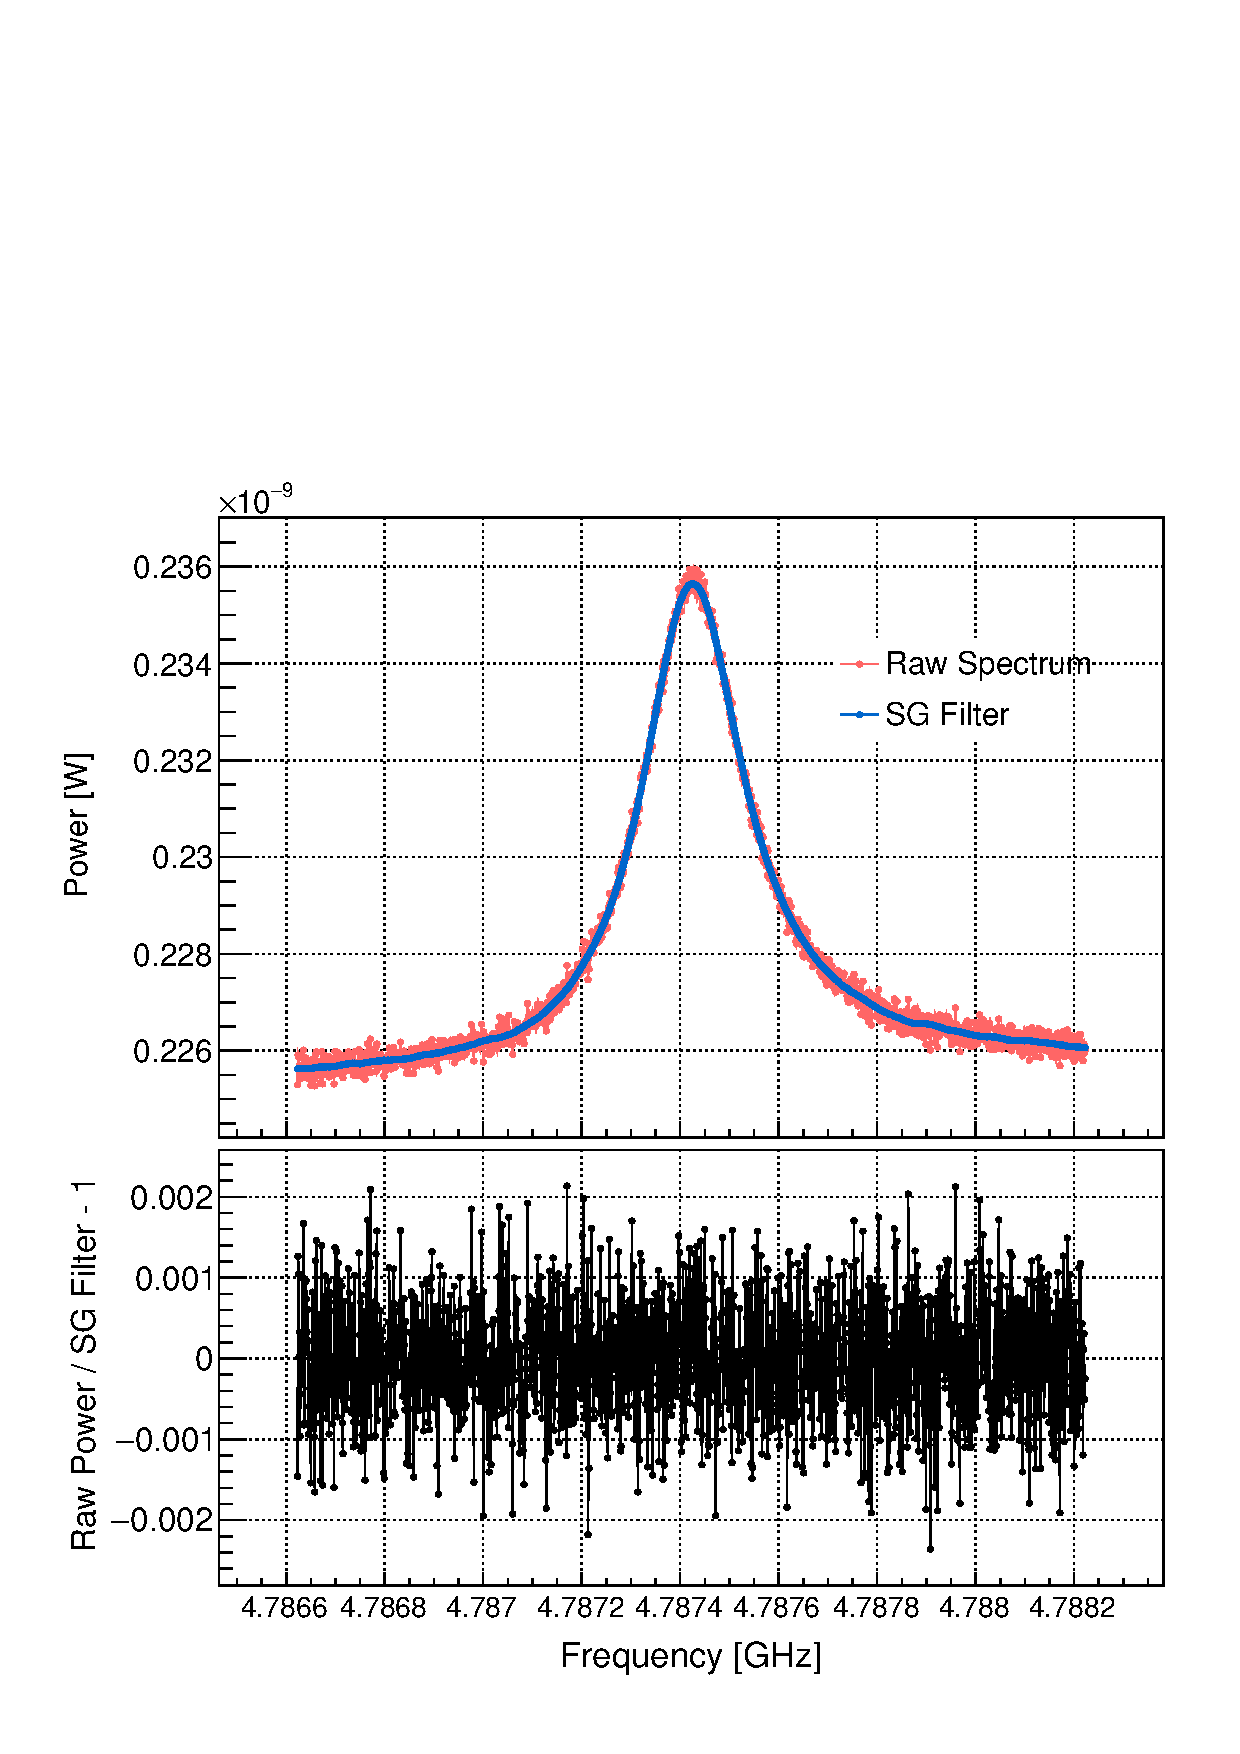
\includegraphics[width=6.5cm]{figures/RawPower_SGPower_Ratio_vs_Freq_Step_0100.pdf}
  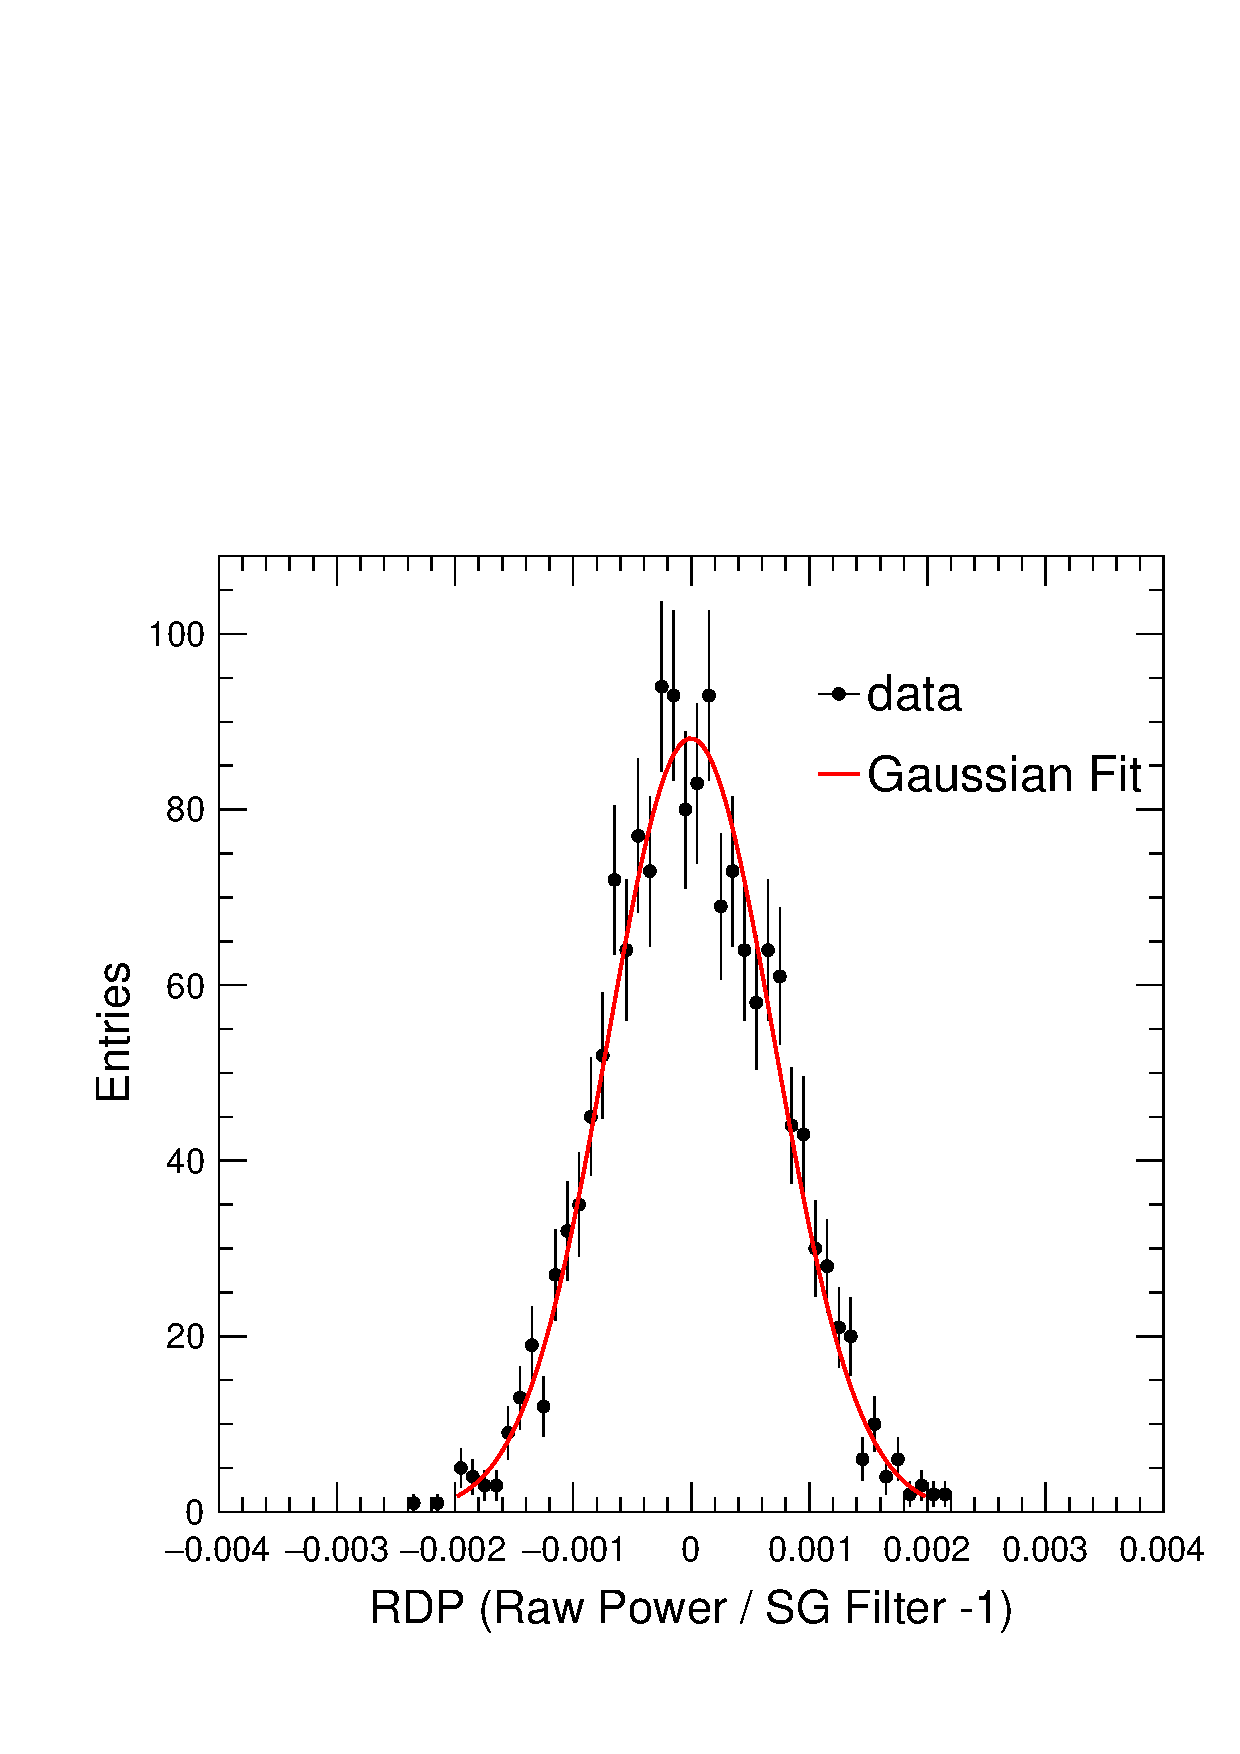
\includegraphics[width=6.5cm]{figures/Histogram_RawPower_SGPower_Ratio_Step_0100.pdf}
  \caption{Upper left panel: The raw averaged power spectrum (red points) and the 
output of the SG filter (blue curve) of one scan. Lower left panel: The normalized 
spectrum,  derived by taking the ratio of the raw spectrum to the SG filter 
and subtracting unity from the ratio. Right plot: Histogram of the normalized spectrum with Gaussian fit.}
  \label{fig:raw_sg_power}
\end{figure}

\begin{figure} [htbp]
  \centering
  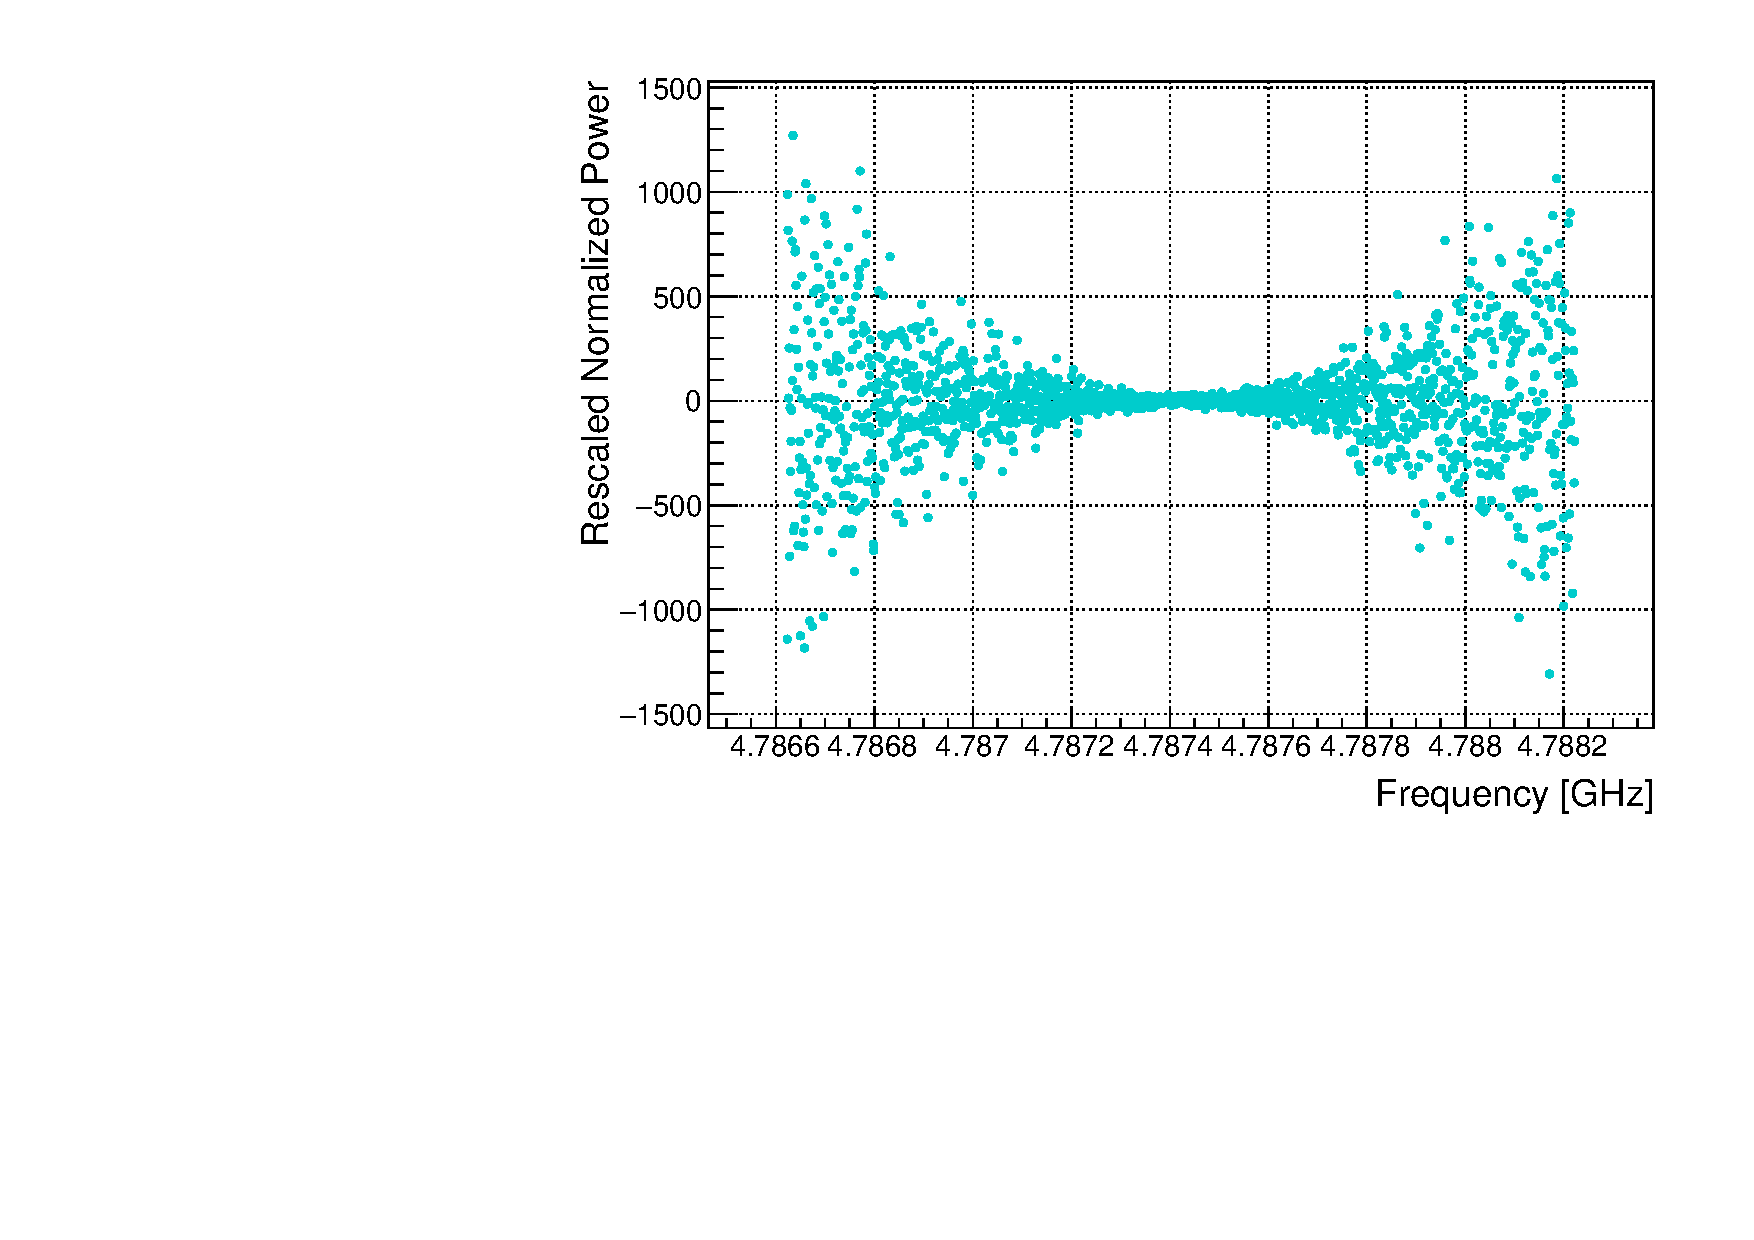
\includegraphics[width=8.6cm]{figures/RescaledPower_vs_Freq_Step_0100.pdf}
  \caption{
  The rescaled spectrum, obtained by multiplying the RDPs in the normalized 
spectrum with the ratio of the system noise power to the expected signal 
power of the KSVZ axion, 
with the Lorentzian response of the cavity taken into account.}
  \label{fig:rescaled_power}
\end{figure}



%First we will choose a window and a order, then move the window and fit the data a with a polynomial with chosen order, it is a kind of generalization  moving average characterized, if the windows is too big, then it will not remove small structures, if it too small, it may kill the signal, you can see that choosing an appropriate window is important, a way to test if the windows are appropriate is to see the system temperature calculated by  $\mu$ and $\sigma$.

%\begin{equation}
%    \label{eq:ts_mu}
%    \mu = k_{B} \cdot T_{S} \cdot \Delta f 
%\end{equation}
%\begin{equation}
%    \label{eq:ts_sigma}
%    \sigma = \frac{k_{B} \cdot T_{S} \cdot \Delta f}{\sqrt{N}}
%\end{equation}

%If we treat the spectrum after the SG filter as a pure noise, we know that the system temperature of a white noise can be calculated by $\mu$ and $\sigma$ (Eq.\eqref{eq:ts_mu}) (Eq.\eqref{eq:ts_sigma}),
%where $k_{B}$ is the Boltzmann constant, $T_{S}$ is the system temperature, $\Delta f$ is the frequency resolution and N is the number of averaging. \\
%If the chosen window is appropriate, the system temperature estimated from $\mu$ and $\sigma$ should be consistent  with each other. \\

%We also did some studies to check if the SG filter removed the axion signal. Assuming a signal bandwidth of 5 kHz, we added the signal into noise spectrum and applied the SG filter. The result shows that the filter does not suppress the axion signal as given in Fig.\ref{fig:weighted_snr}.

%about whether the sg filter will remove the Axion signal, assuming the Axion signal bandwidth is 5KHz, add the signal in a white noise and apply the sg filter , the results show that it will not affect much before and after use, after divide the sg filter result, we will subtract 1 to make the value become 1.

%\begin{figure}[h]
%    \begin{minipage}[h]{.5\textwidth}
%    \centering
%    \includegraphics[width=0.8\textwidth, height = 0.5\textwidth]{Figure/sg_simulation.png}
%    \caption{The simulation for testing the effect of SG filter.}
%    \label{fig:weighted_snr}
%%    \end{minipage}%
%\end{figure}
%\begin{figure}[h]
%    \begin{minipage}[t]{.5\textwidth}
%    \centering
%    \includegraphics[width=0.8\textwidth,height = 0.5\textwidth]{Figure/weighted_snr.png}
%    \caption{Weighed SNR}
%    \label{fig:weighted_snr}
%%    \end{minipage}%
%\end{figure}

\subsection{Combine the spectra with the weighting algorithm} 
\label{sec:weighting_algorithm}

The purpose of the weighting algorithm is to add the spectra from different 
resonant-frequency scans,
 particularly for the frequency bins that appear in multiple spectra.  
Each spectrum was collected with a different cavity resonant frequency. 
Therefore, if a signal appears in a certain frequency bin $j$, due to the
 difference in the resonant frequency and the Lorentzian response, the 
expected signal
 power will be different in each spectrum $i$. The weighting algorithm is 
expected to take this into account with a weight calculated for each bin $j$ of
 the rescaled spectrum $i$, as defined below: %in Eq.~\eqref{eq:weight}:
\begin{equation}
    \label{eq:weight}
    %    {w_{n}}^{i} = \frac{h \cdot p}{(\sigma_{n}^{i})^{2}}
    {w_{ijn}} = \frac{\Gamma_{ijn}}{(\sigma_{ij}^\text{res})^{2}}.
\end{equation}
Note, the symbol $\Gamma_{ijn}=1$ if the $j^\text{th}$ frequency bin in the 
$i^\text{th}$ rescaled spectrum correspond to the same frequency in 
the $n^\text{th}$ bin of the combined spectrum; otherwise, $\Gamma_{ijn}=0$.

The RDP $\delta^\text{com}_{n}$ and the standard deviation 
$\sigma^\text{com}_{n}$ of the $n^\text{th}$ bin in the combined spectrum are 
calculated using Eq.~\eqref{eq:comb_power} and Eq.~\eqref{eq:comb_sigma}, 
respectively. The SNR$^\text{com}_{n}$ is the ratio of 
$\delta^\text{com}_{n}$ to 
$\sigma^\text{com}_{n}$ as given in Eq.~\eqref{eq:comb_snr}. 
%Figure~\ref{fig:power_sigma_comb} and Fig.~\ref{fig:SNR_comb} show the power, 
%the standard deviation, and the SNR of the combined spectrum, respectively.
Figure~\ref{fig:power_sigma_comb} and Fig.~\ref{fig:SNR_comb} show the RDP, 
the standard deviation, and the SNR of the combined spectrum, respectively.

\begin{equation}
    \label{eq:comb_power}
%    \delta_{n}^\text{com} = \frac{ \sum_{1}^{k}\left(\delta_{ij}^\text{res} \cdot {w_{ij}}\right)}{\sum_{1}^{k} {w_{ij}}},
    \delta_{n}^\text{com} = \frac{ \sum\limits_{i}\sum\limits_{j}\left(\delta_{ij}^\text{res} \cdot {w_{ijn}}\right)}{\sum\limits_{i}\sum\limits_{j} {w_{ijn}}},
\end{equation}
\begin{equation}
    \label{eq:comb_sigma}
%    \sigma_{n}^\text{com} = \frac{ \sqrt{\sum_{1}^{k}(\sigma_{ij}^\text{res} \cdot {w_{ij}})^2}}{\sum_{1}^{k} {w_{ij}}},
    \sigma_{n}^\text{com} = \frac{ \sqrt{\sum\limits_{i}\sum\limits_{j}(\sigma_{ij}^\text{res} \cdot {w_{ijn}})^2}}{\sum\limits_{i}\sum\limits_{j} {w_{ijn}}},
\end{equation}
\begin{equation}
    \label{eq:comb_snr}
%    \text{SNR}_{n}^\text{com} = \frac{\delta^\text{com}_{n}}{\sigma^\text{com}_{n}}= \frac{\sum_{1}^{k}\left(\delta_{ij}^{res} \cdot {w_{ij}}\right)}{ \sqrt{\sum_{1}^{k}(\sigma_{ij}^{res} \cdot {w_{ij}})^2}},
    \text{SNR}_{n}^\text{com} = \frac{\delta^\text{com}_{n}}{\sigma^\text{com}_{n}}= \frac{\sum\limits_{i}\sum\limits_{j}\left(\delta_{ij}^{res} \cdot {w_{ijn}}\right)}{ \sqrt{\sum\limits_{i}\sum\limits_{j}(\sigma_{ij}^{res} \cdot {w_{ijn}})^2}}.
\end{equation} 
For each bin $n$ in the combined spectrum, there are $m_n$ non-vanishing 
contributions to the sums above. The value of $m_n$ ranges from 2 to 26; 
in general the leftmost bin or the bin with the smallest frequency 
(the rightmost bin or the bin with the highest frequency) in each scan has 
the minimum (maximum) number of $m_n$. 


\begin{figure}[h]
    \centering
    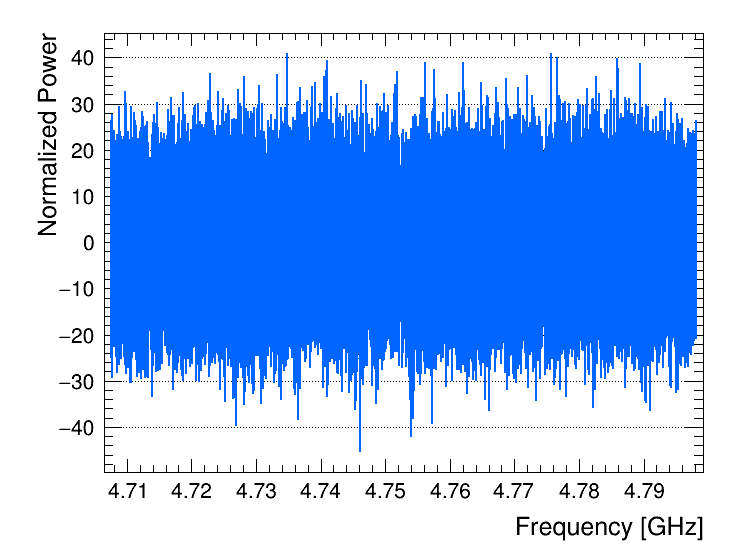
\includegraphics[width=8.6cm]{figures/Power_CombSpectrum_AxionRun_AllSteps_Rescan_SG4_W201_LqWeight.png}
    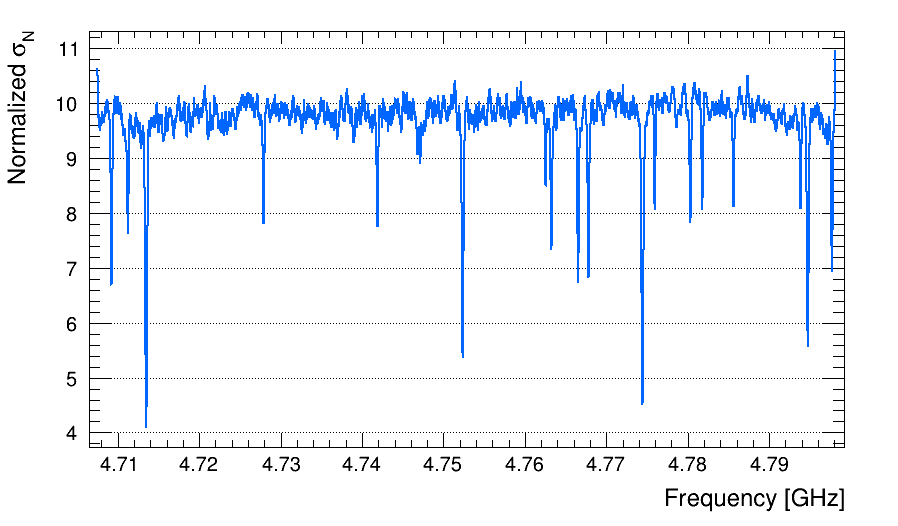
\includegraphics[width=8.6cm]{figures/Sigma_CombSpectrum_AxionRun_AllSteps_Rescan_SG4_W201_LqWeight.png}
    \caption{The combined RDP $\delta$ following Eq.~\eqref{eq:comb_power} 
(upper) and the standard deviation $\sigma$ derived from 
Eq.~\eqref{eq:comb_sigma} (lower).}
    \label{fig:power_sigma_comb}
\end{figure}

\begin{figure}[hbt!]
    \centering
    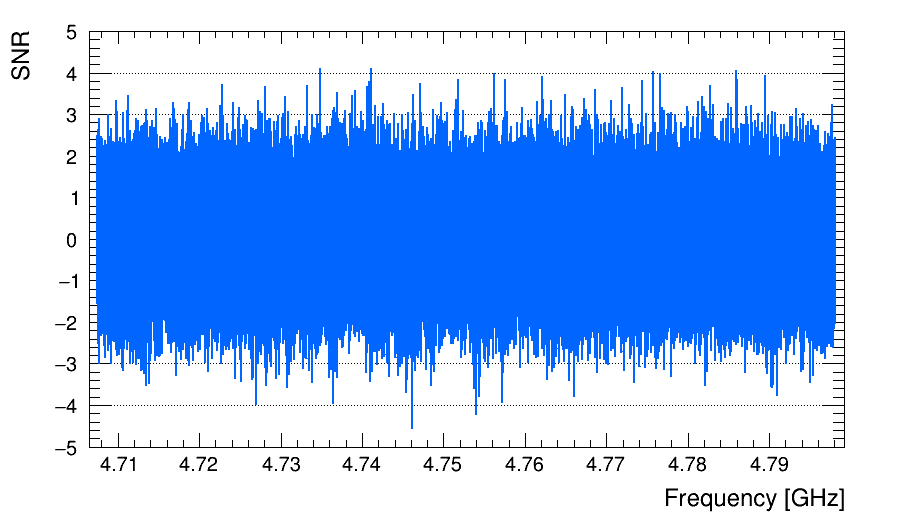
\includegraphics[width=8.6cm]{figures/SNR_CombSpectrum_AxionRun_AllSteps_Rescan_SG4_W201_LqWeight.png}
    \caption{The signal-to-noise ratio (SNR) calculated using 
Eq.\eqref{eq:comb_snr} of the combined spectrum. }
    \label{fig:SNR_comb}
\end{figure}


%where ${\delta_n^i}$ and ${\sigma_n^i}$ are the measured power and the corresponding standard deviation of the ${n^{\mathrm{th}}}$ frequency bin of the ${i^{\mathrm{th}}}$ spectrum., From the weighted power in ${n^{th}}$ bin in Eq.\eqref{eq:weighted_power}, and weighted $\sigma$ in Eq.\eqref{eq:weighted_sigma}, we can get our Signal to noise ratio as Eq.\eqref{eq:weighted_SNR}

\subsection{Merge bins}
\label{sec:merge}

The expected axion bandwidth is about 5~kHz at the frequency of $\approx5$~GHz. 
In this paper, the interested frequency range is \flo -- \fhi~GHz and the bin 
width is 1~kHz. Therefore, in order to maximize the SNR, a running window of 
five consecutive bins in the combined spectrum is applied and the five bins 
within each window are merged to construct a final spectrum.
The purpose of using a running window is to avoid the signal power broken 
into different neighboring bins of the merged spectrum. 
%Before defining the 
%weights for merging, 
%the power and the standard deviation of each bin in the combined spectrum are 
%multiplied with $M=5$: $\delta^{c}_n \rightarrow M\delta^\text{com}_n$ and 
%$\sigma^{c}_n \rightarrow M \sigma^\text{com}_n$. This rescaling gives the 
%expected mean of the normalized power $\mu^\text{com}_k = 1$ if a KSVZ axion 
%signal power leaves a fraction 1/$M$ of its power in the $k^\text{th}$ 
%bin of the combined spectrum.
Due to the nonuniform distribution of the axion signal 
[Eq.~\eqref{eq:simplesignal}],
the contributing bins need to be rescaled to have the same RDP, of which the 
standard deviation is used to define the maximum likelihood (ML)
weight for merging. The rescaling is performed by dividing the 
$\delta^\text{com}_{g+k-1}$ and $\sigma^\text{com}_{g+k-1}$ in the combined 
spectrum by an integral of the signal line shape $L_{k}$ 
[Eq.~\eqref{eq:Lq_integral}]: 
\begin{equation}
  \label{eq:rescaled_delta_sigma_com}
  \begin{split}
  \delta^\text{rs}_{g+k-1} = \frac{\delta^\text{com}_{g+k-1}}{L_{k}},\\
  \sigma^\text{rs}_{g+k-1} = \frac{\sigma^\text{com}_{g+k-1}}{L_{k}}.
  \end{split}
\end{equation}
Here, the $\delta^\text{rs}_{g+k-1}$ and $\sigma^\text{rs}_{g+k-1}$ are the 
rescaled RDP and standard deviation that will be used later for merging. The 
variable $g = 1,..,N-M+1$ is the index for the frequency bins in the final 
spectrum and $k = 1,..,M$, in which $M = 5$ is the number of merged bin in 
this analysis. The numbers $N$ and $N-M+1$ are the total numbers of bins in 
the combined and final spectrum, respectively. The integral $L_{k}$ is 
defined as: 
\begin{equation}
  \label{eq:Lq_integral}
  L_{k} = \int_{f_a +\delta f_m + (k-1)\Delta f_\text{bin}}^{f_a +\delta f_m + k\Delta f_\text{bin}} \mathcal{F}(f) \,df,
\end{equation}
where the frequency $f_a=\left.\ma c^2\middle/h\right.$ is the axion 
frequency, $\delta f_m$ is the misalignment between $f_a$ and the lower
boundary of the $g^\text{th}$ bin in the combined spectrum.
The function $\mathcal{F}(f)$ has been defined in Eq.~\eqref{eq:simplesignal}. 
The misalignment effect as mentioned in the HAYSTAC paper ~\cite{HAYSTACII} 
has been studied and the results of the \gagg\ limits are found to be 
insensitive to this effect. 

%The rescaled $\delta^\text{com}_{g+k-1}$ and $\sigma^\text{com}_{g+k-1}$ and 
%ML weight are defined:


%In order to get misalignment-independence line shape, the average ($L\bar_{k}$) of
%$L_{k}(\delta f_m)$ over the range $\delta f_m$ is used.
%The range of $\delta f_m$ is defined $-z \Delta f_\text{bin} < \delta f_m < (1-z) \Delta f_\text{bin}$,
%with $0 < z < 1$. 

%Then the maximum likelihood weights, defined in Eq.~\eqref{eq:merge_weight} 
%based on the Maxwellian line shape for axions [Eq.~\eqref{eq:simplesignal}], 
%are used to build the merged spectrum: 
The ML weight is defined as: 
\begin{equation}
    \label{eq:merge_weight}
    w_{gk} = \frac{1}{(\sigma_{g+k-1}^\text{rs})^{2}} = \frac{L_{k}^{2}}{(\sigma_{g+k-1}^\text{com})^{2}},
\end{equation}

% in which 
%\begin{equation}
%    \label{eq:Lq_integtal}
%    L_{k} = \int_{f_a +\delta f_m + (k-1)\Delta f_\text{bin}}^{f_a +\delta f_m + k\Delta f_\text{bin}} \mathcal{F}(f) \,df. 
%\end{equation}
%Here, $g = 1,..,N-M+1$ is the index for 
%the frequency bins in the final spectrum and $M=5$ is the number of merged 
%bins. 
%The total number of bins in the combined (final merged) spectrum is
%$N$ ($N-M+1$). 
%The variable $k$ is the index within the group of bins for merging and 
%$k = 1,..,M$. 
%The frequency $f_a=\left.\ma c^2\middle/h\right.$ is 
%the axion frequency, $\delta f_m$ is the misalignment between $f_a$ and the lower 
%boundary of the $g^\text{th}$ bin in the combined spectrum. 

%where $L_q$ is the integral of the line shape from the lower edge to higher 
%edge of ${q^{th}}$ bin. 

%We have a weight Eq.\eqref{eq:merge_weight}, where Lq is the area in ${q^{th}}$ bin and $\sigma_{q}$ is the weighted $\sigma$ in the $q^{\mathrm{th}}$ bin , Eq.\eqref{eq:axion_line_shape} is the axion CDM(cold dark matter) line shape, where $\big \langle \beta^{2} \big \rangle = \big \langle v^{2} \big \rangle /c^{2}$ and $\big \langle v^{2} \big \rangle = (270km/s)^{2}\ , \big \langle v^{2} \big \rangle$ is the squared virial velocity. Eq.\eqref{eq:L_q_integtal},

The RDP, the standard deviation, and the SNR of the merged spectrum are:

\begin{equation}
    \delta_{g}^\text{merged} = \frac{ \sum\limits_{k = 1}^{M}\left(\delta_{g+k-1}^\text{rs} \cdot {w_{gk}}\right)}{\sum\limits_{k = 1}^{M} {w_{gk}}} = \frac{\sum\limits_{k = 1}^{M}\frac{\delta_{g+k-1}^\text{com}}{L_{k}} \cdot \left(\frac{L_{k}}{\sigma_{g+k-1}^\text{com}}\right)^2} {\sum\limits_{k = 1}^{M}\left(\frac{L_{k}}{\sigma_{g+k-1}^\text{com}}\right)^2},
    \label{eq:merged_power}
\end{equation}

\begin{eqnarray}
  \sigma_{g}^\text{merged} & =  & \frac{ \sqrt{\sum\limits_{k = 1}^{M} \left(\sigma_{g+k-1}^\text{rs} \cdot {w_{gk}}\right)^2}}{\sum\limits_{k = 1}^{M} {w_{gk}}} = \frac{\sqrt{\sum\limits_{k = 1}^{M} \left(\frac{L_{k}}{\sigma_{g+k-1}^\text{com}}\right)^2}}{\sum\limits_{k = 1}^{M} \left(\frac{L_{k}}{\sigma_{g+k-1}^\text{com}}\right)^2}  \nonumber \\
    & = & \frac{1}{\sqrt{\sum\limits_{k = 1}^{M} \left(\frac{L_{k}}{\sigma_{g+k-1}^\text{com}}\right)^2}}
    \label{eq:merged_sigma}
\end{eqnarray}

\begin{equation}
    \label{eq:merged_snr}
    %    \text{SNR}_{g}^\text{merged} = \frac{\delta^\text{merged}_{g}}{\sigma^\text{merged}_{g}} = \frac{\sum\limits_{k = 1}^{M}\left(\delta_{g+k-1}^\text{com} \cdot {w_{gk}}\right)}{ \sqrt{\sum\limits_{k = 1}^{M} \left(\sigma_{g+k-1}^\text{com} \cdot {w_{gk}}\right)^2}},
    \text{SNR}_{g}^\text{merged} = \frac{\delta^\text{merged}_{g}}{\sigma^\text{merged}_{g}} = \frac{\sum\limits_{k = 1}^{M}\frac{\delta_{g+k-1}^\text{com}}{L_{k}} \cdot \left(\frac{L_{k}}{\sigma_{g+k-1}^\text{com}}\right)^2}{\sqrt{\sum\limits_{k = 1}^{M} \left(\frac{L_{k}}{\sigma_{g+k-1}^\text{com}}\right)^2}}
\end{equation}

%For the flat distribution, $L_{k}$ is normalized by the number of merged bins 
%to have the expected power excess of 1 for KSVZ signal.

%where $M=5$ is the number of merged bins. $g = 1,..,N-M+1$ is the index for 
%the frequency bins in the final spectrum.  
%The total number of bins in the combined (final merged) spectrum is 
%$N$ ($N-M+1$). 
%Without the multiplication factor $M$ in 
%Eqs.~\eqref{eq:merged_power}--~\eqref{eq:merged_sigma}, the results of the two equations 
%simply provide the weighted averages of RDP and standard deviation, respectively.   
%Assuming that the axion signal leaves a fraction $1/M$ of its power in one 
%frequency bin, adding the factor $M$ converts the average into a summation of the values in the 
%five bins and can recover the full size of the axion signal. 

%Adding adjacent bin with a weight Eq.\eqref{eq:merged_power} Eq.\eqref{eq:merged_sigma}, where k is the number of adjacent bin to be merged, q is ${q^{th}}$ merged bin, with Eq.\eqref{eq:merged_sigma}, we can get our weighted merged power spectrum FIG.\ref{fig:merged_data}.


\subsection{Rescan and set limits on \gagg} 
Before the collection of the CD102 data, a 5$\sigma$ SNR target was chosen, 
which corresponds to a candidate threshold of 3.355$\sigma$ at 95\% confidence.
 After the merging as described in Sec.~\ref{sec:merge}, if there were 
any potential signal with an SNR larger than 
3.355, a rescan would be proceeded to check if it were a real signal 
or a statistical fluctuation. 
The procedure of the CD102 data taking was to perform a rescan after 
covering every 10~MHz; the rescan was done by adjusting the tuning rod of the 
cavity so to match the resonant frequency to the frequency of the candidate. 
In total, 22 candidates with an SNR greater than 3.355 were found. 
Among them, 17 candidates were from the fluctuations because they were gone 
after a few rescans. 
The remaining five candidates, in the frequency ranges of 
4.710170 -- 4.710190~GHz and 4.747301 -- 4.747380~GHz, reached an SNR greater than 
4 after rescanning. The signals in the second frequency 
range were detected via a portable antenna outside the DR and found 
to come from the instruments in the laboratory, while the signals 
in the first frequency range were weaker but still present after 
turning off the external magnetic field. 
Therefore, these five candidates are considered external signals and 
no limits are placed for the above two frequency ranges.  
More details can be found in the 
TASEH instrumentation paper~\cite{TASEHInstrumentation}. 
Figure~\ref{fig:power_sigma_merged} and Fig.~\ref{fig:SNR_merged} show the 
RDP, the standard deviation, and the SNR of the merged spectrum after 
including data from both the original scans and the rescans, respectively. 

Since no candidates were found after the rescan, an upper limit on 
the signal power $P_s$ is derived by setting $P_s$ equal to 
$5\sigma_{g}^\text{merged}\times P_{g}^\text{KSVZ}$, where 
the $\sigma_{g}^\text{merged}$ and $P_{g}^\text{KSVZ}$ are 
the standard deviation and the expected signal power for the KSVZ axion 
for a certain frequency bin $g$ in the merged spectrum. 
Then, the 95\% C.L. limits on the dimensionless parameter 
\ggamma\ and the axion-two-photon coupling \gagg\ could be derived 
according to Eq.~\eqref{eq:ps} and Eq.~\eqref{eq:grelation}. 
See Sec.~\ref{sec:results} for the final limits including the systematic 
uncertainties.

\begin{figure}[h]
    \centering
    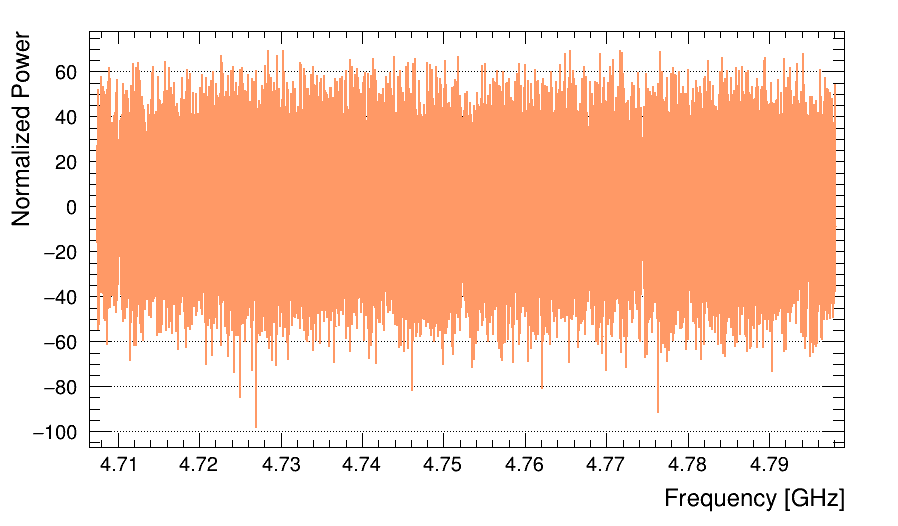
\includegraphics[width=8.6cm]{figures/Power_GrandSpectrum_AxionRun_AllSteps_Rescan_Merged_5bin_SG4_W201_LqWeight.png}
    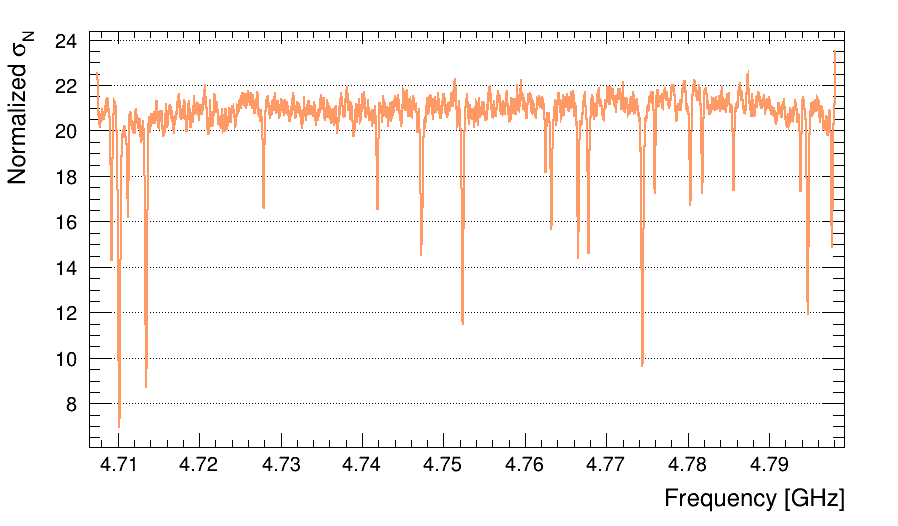
\includegraphics[width=8.6cm]{figures/Sigma_GrandSpectrum_AxionRun_AllSteps_Rescan_Merged_5bin_SG4_W201_LqWeight.png}
    \caption{The merged RDP $\delta$ following Eq.~\eqref{eq:merged_power} 
(upper) and the standard deviation $\sigma$ derived from Eq.~\eqref{eq:merged_sigma} (lower). The results shown are obtained using data from both the 
original scans and the rescans.}
    \label{fig:power_sigma_merged}
\end{figure}

\begin{figure}[hbt!]
    \centering
    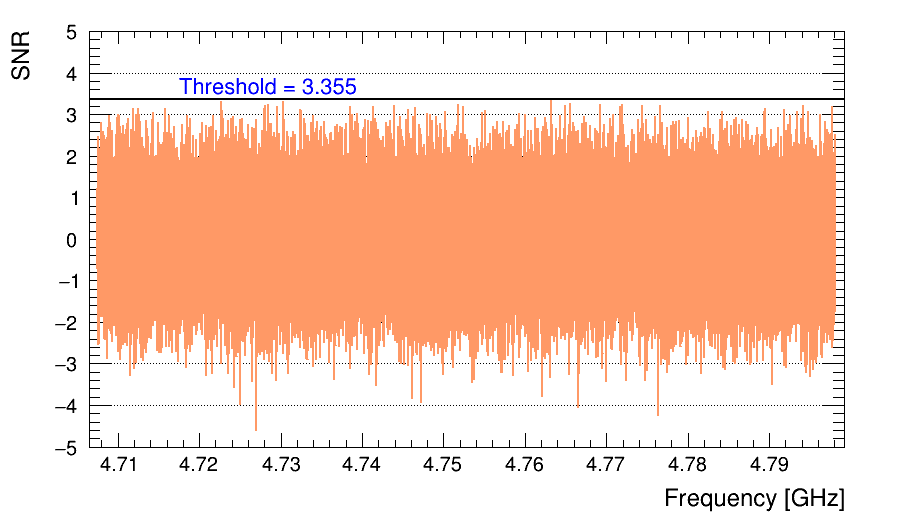
\includegraphics[width=8.6cm]{figures/SNR_GrandSpectrum_AxionRun_AllSteps_Rescan_Merged_5bin_SG4_W201_LqWeight.png}
    \caption{The signal-to-noise ratio (SNR) calculated using Eq.~\eqref{eq:merged_snr} for the merged spectrum including data from both the original 
scans and the rescans. No candidate exceeds the threshold of 
$3.355\sigma$ (solid-black horizontal line). }
    \label{fig:SNR_merged}
\end{figure}

\section{Analysis of the Synthetic Axion Data}\label{sec:faxion}
After TASEH finished collecting the CD102 data on November 15, 2021, 
the synthetic axion signals were injected into the cavity and read out via the 
same transmission line and amplification chain. The procedure 
to generate axion-like signals is summarized in 
Ref.~\cite{TASEHInstrumentation}. 
%Due to the uncertainties on the losses of signal transmission
% lines, the synthetic axion signals are not used to perform an absolute 
%calibration of the search sensitivity. Instead, 
A test with synthetic axion signals could be used to verify the procedures of 
data acquisition and physics analysis. The synthetic axion signals 
have a wider width (8~kHz) and longer tails compared to the line shape 
described by Eq.~\eqref{eq:simplesignal}. The total signal power injected 
corresponds to $\ggamma\approx 20 \left|g_\text{KSVZ}\right|$. 
The SNR of the frequency bin with maximum power ($\approx 11\%$ of the 
total signal power), 
%synthetic axion signals, at 4.708970~GHz, was set to $\approx 3.35$.%, 
 at 4.70897~GHz, was set to $\approx 3.35$. 
%corresponding to a power of $\approx 6.03 \times 10^{-13}$~W in a 1-kHz 
%frequency bin.  

The same analysis procedure as described in Sec.~\ref{sec:ana} is applied 
to the data with synthetic axion signals. 
Figure~\ref{fig:faxionstep} presents the individual raw power spectra in 
the 24 frequency scans. Before combining 
the 24 spectra, the SNR of the maximum-power bin from the scan with a resonant 
frequency closest to the injected signal is measured to be 
3.58. %the SNR is slightly higher than 3.35 due to a 
%5\% difference in the noise fluctuation between the measurements from 
%the calibration and the measurements taken right before injecting 
%axion-like signals. 
After the combination of the spectra and the merging of five frequency 
bins, the SNRs of the maximum-power bin increase to 4.74 and 6.12, 
respectively. Figure~\ref{fig:faxioncombinemerge} presents 
the SNR after the combination and the merging, respectively.    
%the 24 scans of the 
%synthetic axion data and the two 
%scans of the CD102 data are included and processed together. 
%
In order to 
validate the results of the SNRs, the analysis procedure is also applied  
to the simulated spectra that include both noise and a signal with the 
same power and the same line shape as those of the injected synthetic axions. 
The SNRs obtained with 200 simulations, before 
the combining, after the combining, and after the merging are %4.51 +/- 0.56% 
%3.56 +/- 0.47, 6.88 +/- 0.78
$3.6\pm 0.5$, $4.5\pm0.6$, and $6.9\pm0.8$, respectively, 
which are 
consistent with the results from the synthetic axion data.  
%In addition to the 
%injected synthetic axion signal, a candidate at 4.70801~GHz is found after 
%merging the spectra. Due to the limited access to the DR, 
%it is not possible to perform a rescan after the collection of the 
%synthetic axion data. Therefore,  
%the CD102 data from the two scans that had resonant frequencies close to 
%the candidate frequency are added so to mimic the rescan; the candidate is 
%found to be a statistical fluctuation.  
%Figures~\ref{fig:faxioncombine}--~\ref{fig:faxionmerge} present 
%the RDP spectra with the corresponding SNR, respectively, after combining 
%The analysis results of the synthetic axion signals prove that a power 
%excess of more than 5$\sigma$ can be found at the expected frequencies via 
%the standard analysis procedure. 
The consistency of the SNRs demonstrates 
the capability of the experimental setup and the analysis strategy to discover 
an axion signal with 
$\ggamma\approx {\cal O}\left(10\left|g_\text{KSVZ}\right|\right)$.


\begin{figure}[htbp]                                                                                                  
    \centering                                                                                                                       
    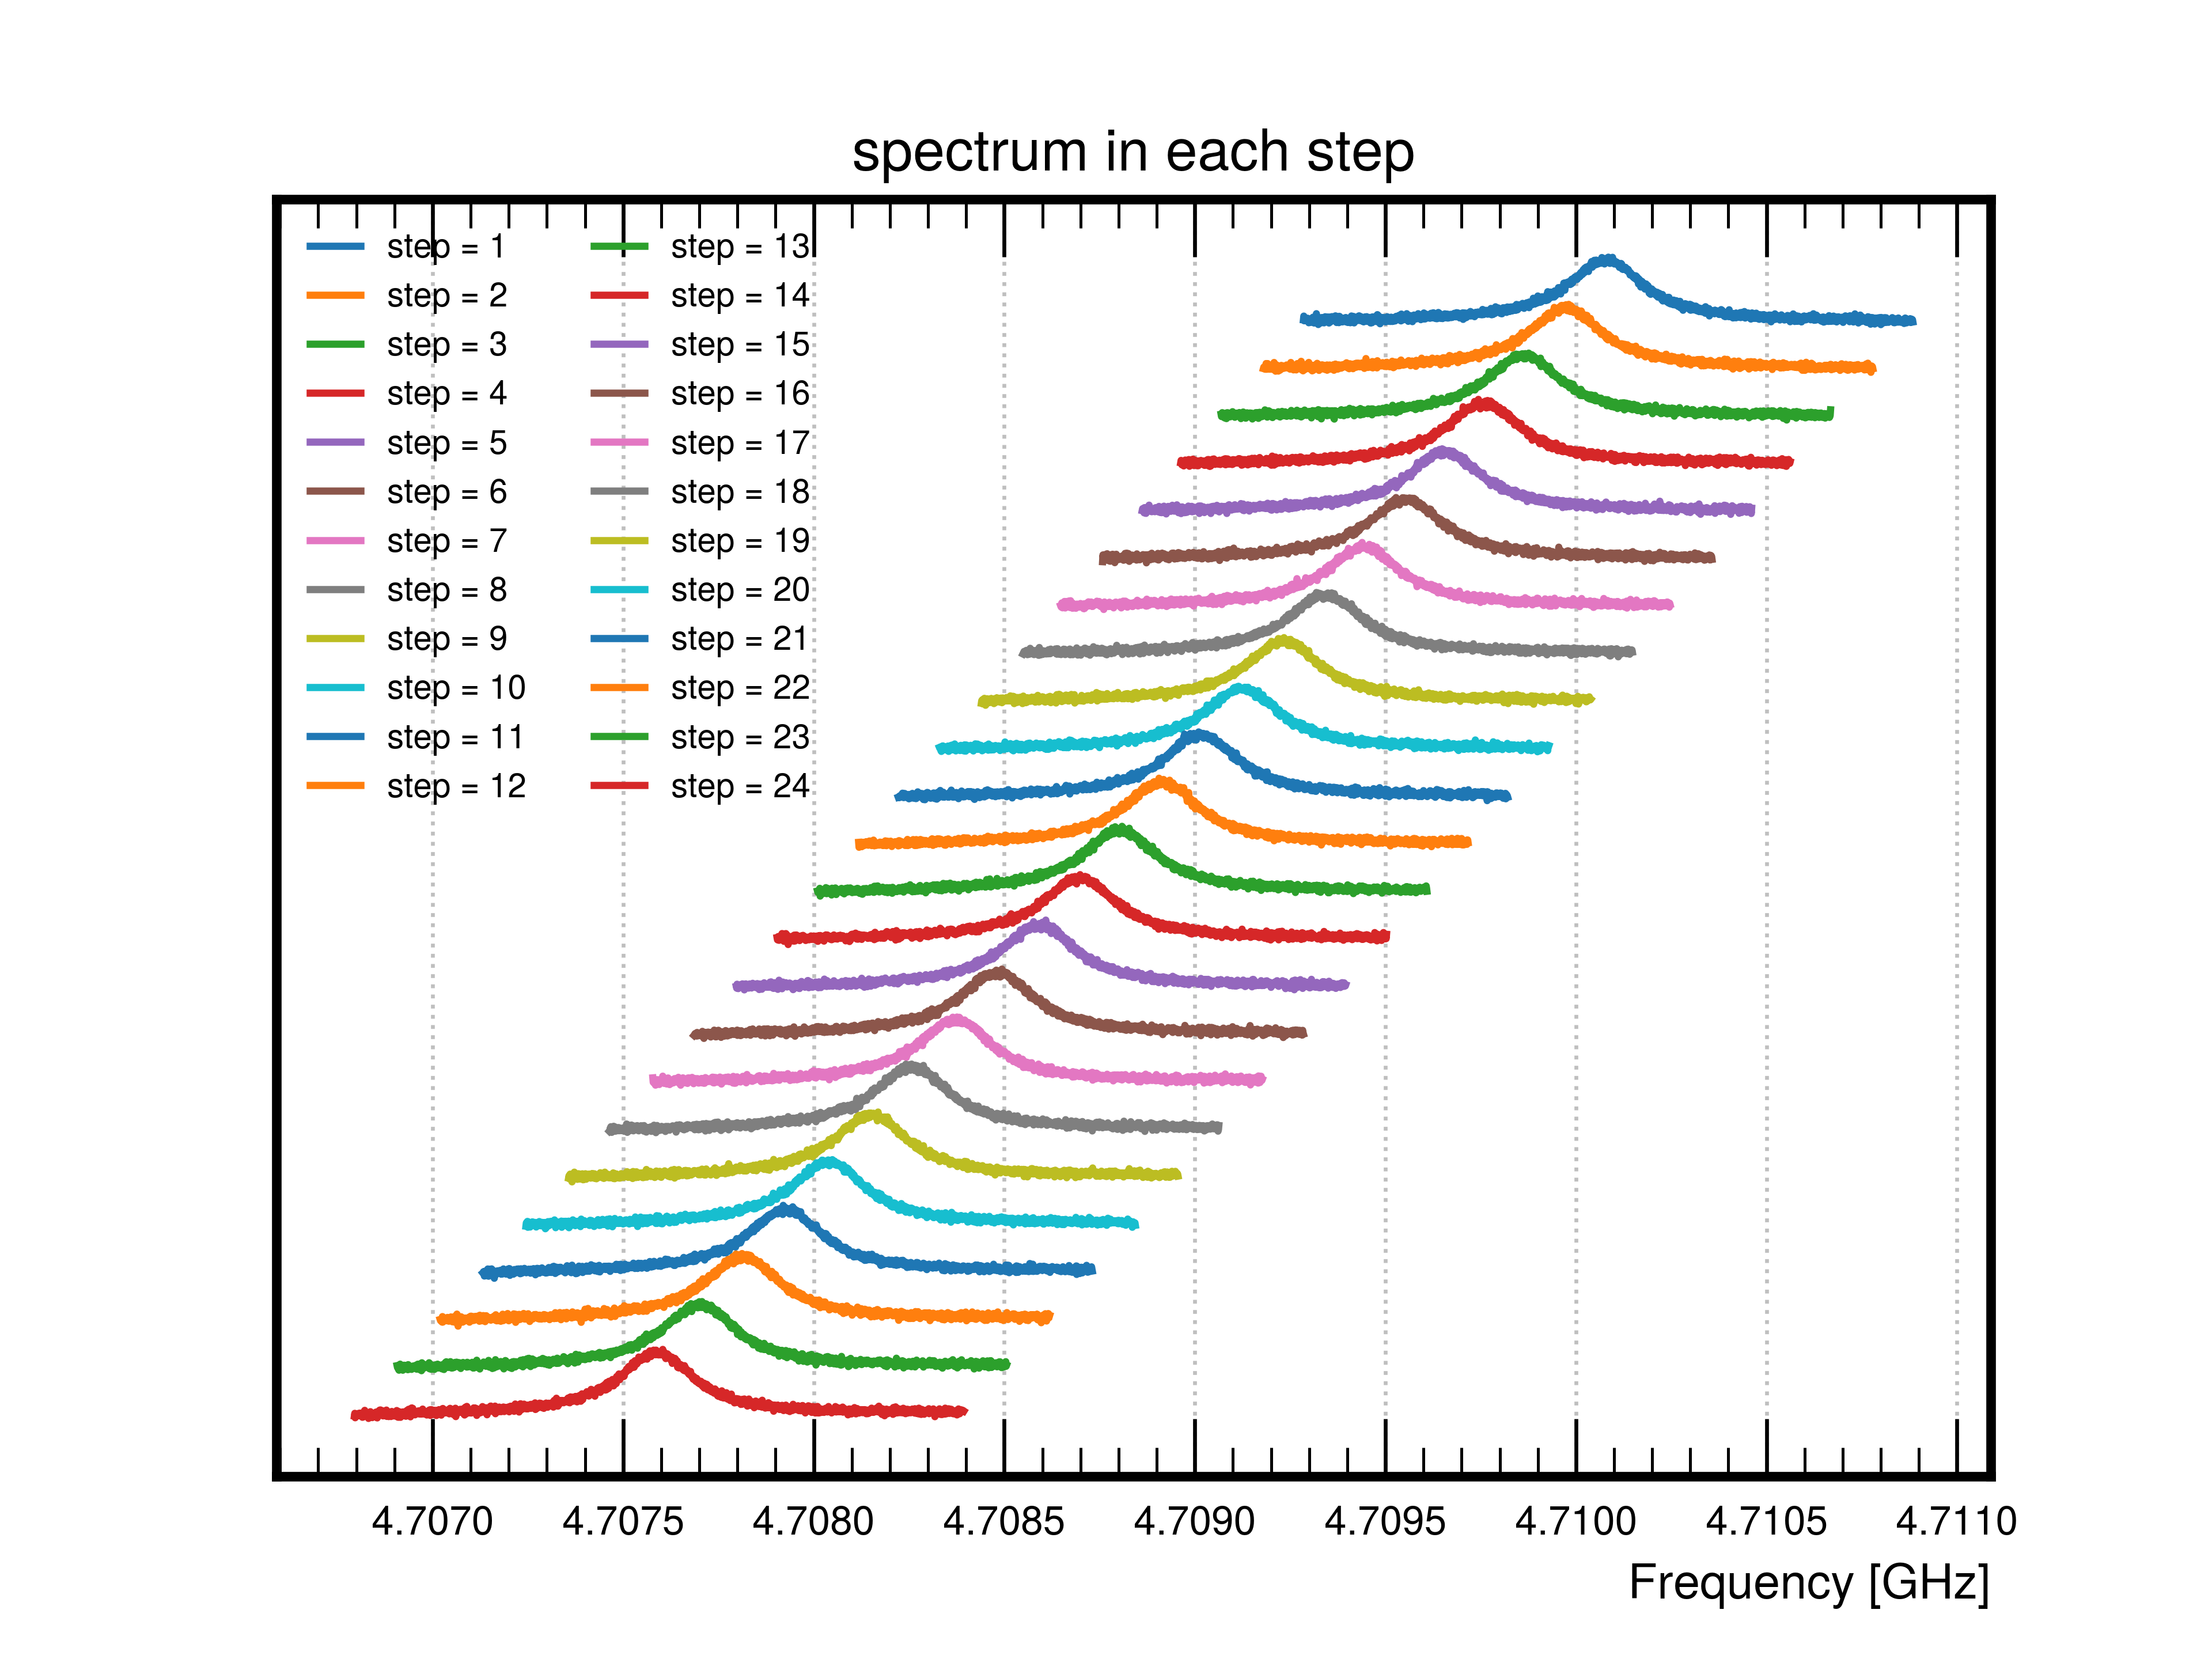
\includegraphics[width=8.6cm]{figures/faxion_rawpower_24steps.png}
 \caption{The raw output power spectra, before applying the 
 SG filter, from the 24 frequency steps of the synthetic axion 
data. In order to show the spectra clearly, the spectra are shifted 
with respect to each other with an arbitrary offset in the vertical scale.}                
\label{fig:faxionstep}                                                                                                            
\end{figure}                       

%\begin{figure}[htbp]                                                                                                  
%    \centering                                                                                                                       
%    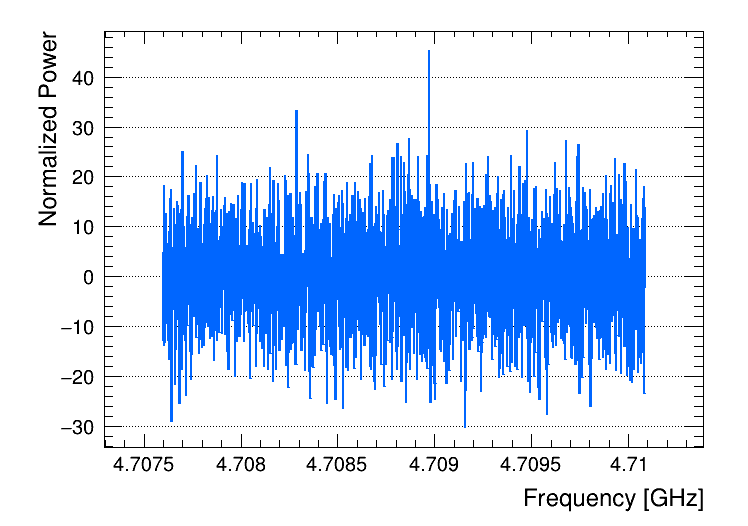
\includegraphics[width=8.6cm]{figures/Power_CombSpectrum_FaxionRun_AllSteps_Rescan_SG4_W201.png}
%    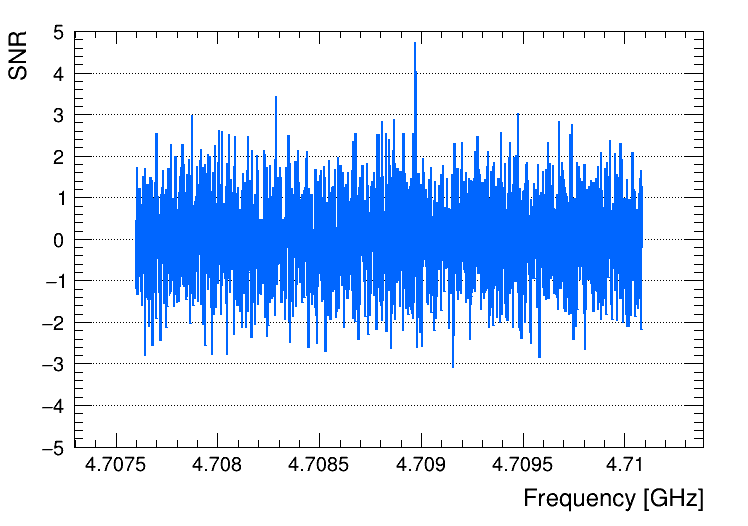
\includegraphics[width=8.6cm]{figures/SNR_CombSpectrum_FaxionRun_AllSteps_Rescan_SG4_W201.png}
%    \caption{The RDP (upper) and the 
%signal-to-noise ratio (lower) after combining the spectra 
%of the synthetic axion data with overlapping frequencies from different scans.
% The procedure and the weights for combination are summarized in 
%Sec.~\ref{sec:weighting_algorithm}.}                
%\label{fig:faxioncombine} 
%\end{figure}                       


%\begin{figure}[htbp]                                                   
%\centering                                                                                                                       
%   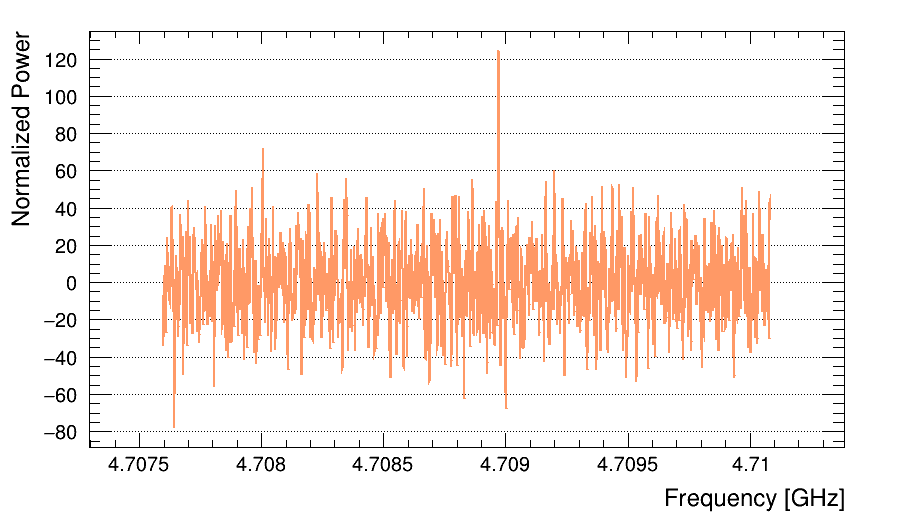
\includegraphics[width=8.6cm]{figures/Power_GrandSpectrum_FaxionRun_AllSteps_Rescan_Merged_5bin_SG4_W201_LqWeight.png}
%    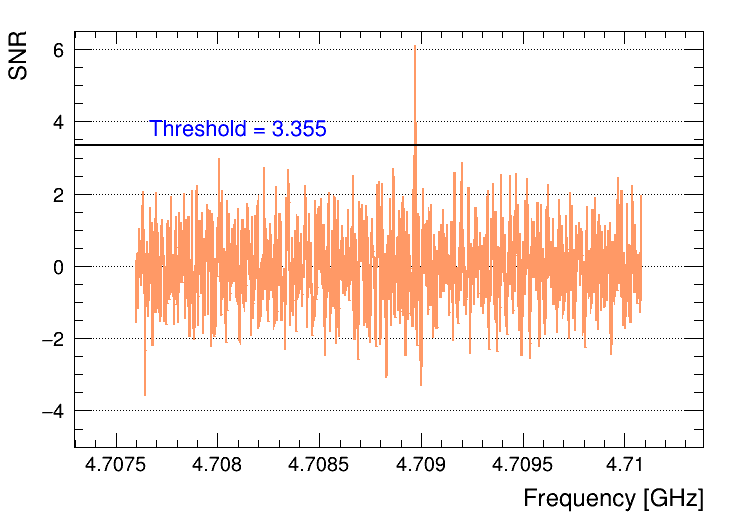
\includegraphics[width=8.6cm]{figures/SNR_GrandSpectrum_FaxionRun_AllSteps_Rescan_Merged_5bin_SG4_W201_LqWeight.png}
%    \caption{The RDP (upper) and the signal-to-noise ratio (lower) after 
%merging the RDP measured in five neighboring frequency bins of the 
%synthetic axion data. 
%The procedure and the weights for merging 
%are summarized in Sec.~\ref{sec:merge}.}                
%\label{fig:faxionmerge}    
%\end{figure}                       



\begin{figure}[htbp]                                                                                                  
    \centering                                                                                                                       
    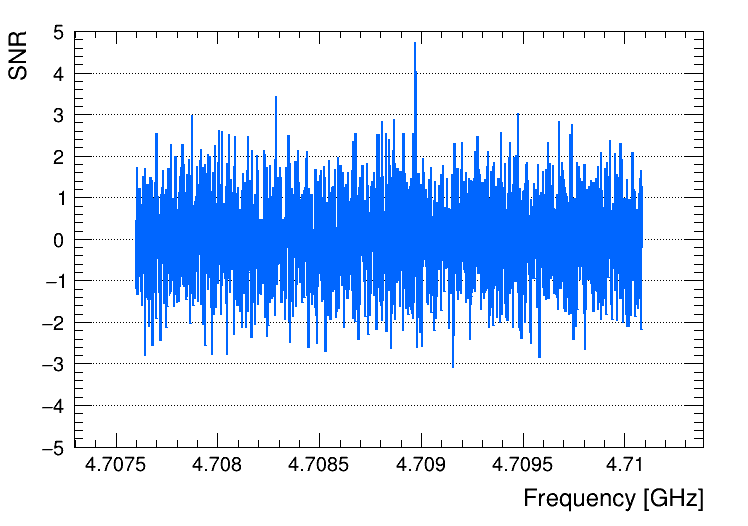
\includegraphics[width=8.6cm]{figures/SNR_CombSpectrum_FaxionRun_AllSteps_Rescan_SG4_W201.png}
    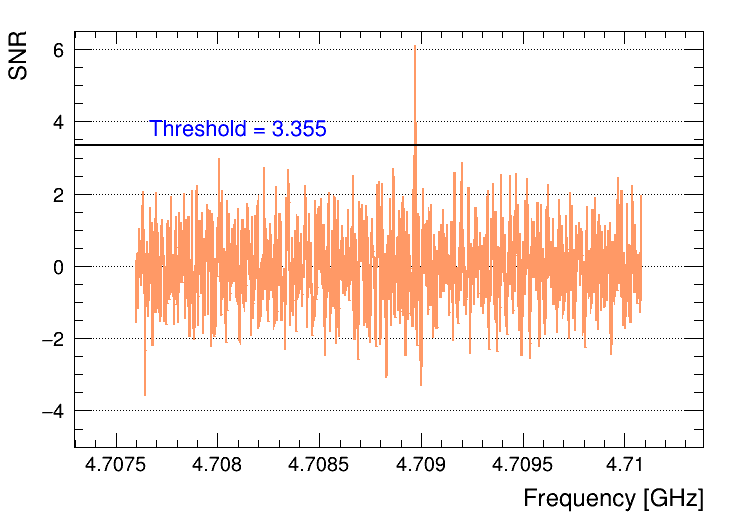
\includegraphics[width=8.6cm]{figures/SNR_GrandSpectrum_FaxionRun_AllSteps_Rescan_Merged_5bin_SG4_W201_LqWeight.png}
    \caption{The signal-to-noise ratio, from the synthetic axion data, 
after combining the spectra with overlapping frequencies from different 
scans (upper) and after merging the RDP measured in five neighboring 
frequency bins (lower). 
The procedure and the weights for combination and merging are summarized in 
Sec.~\ref{sec:weighting_algorithm} and Sec.~\ref{sec:merge}, respectively.}               
\label{fig:faxioncombinemerge} 
\end{figure}                       

   

\section{Systematic Uncertainties} \label{sec:sys}
The systematic uncertainties on the \gagg\ limits arise from the 
following sources:
\begin{itemize}
\item Uncertainty on the product 
$\left.Q_L\beta\middle/\left(1+\beta\right)\right.$ in Eq.~\eqref{eq:ps}: 
In order to extract the loaded quality factor $Q_L$ and the coupling 
coefficient $\beta$, a fitting of the measured results of the cavity 
scattering matrix was performed. A relative uncertainty of 3.6\% is 
assigned to this product, after a comparison of the measurements at 
$T_\text{c}\simeq155$~mK with a prediction extrapolated from the measurements 
at room temperature. More details about the measurements of the 
cavity properties can be found in Ref.~\cite{TASEHInstrumentation}. 
A 3.6\% variation of this product results in a 1.9\% uncertainty 
on the \gagg\ limits. 

\item Uncertainties on the noise temperature \ta\ from: (i) the RMS of 
the measurements in the calibration: 
$\left. \Delta \ta\middle/\ta\right.= 2.3\%$,  
%(see Sec.~\ref{sec:calibration} and Fig.~\ref{fig:hemtcalvsf}).
%
%\item Uncertainty on the noise temperature \ta\ 
and (ii) from the largest difference 
between the value determined by the calibration and that from the CD102 
data: $\left. \Delta \ta\middle/\ta\right.= 4\%$ 
(see Sec.~\ref{sec:calibration} and Fig.~\ref{fig:hemtcalvsf}). 
These two uncertainties on the \ta\ result in a 2.8\% uncertainty 
on the \gagg\ limits. 

%\item Uncertainty on the misalignment $\delta f_m$ between the true 
%axion frequency $f_a$ and the lower bin boundaries in the merged spectrum 
%(see Sec.~\ref{sec:merge}).
\item Uncertainty due to the misalignment (see Sec.~\ref{sec:merge}):
  estimated by comparing the central results to the one without misalignment
  ($\delta f_m = 0$)
  and to the ones with given values of $\delta f_m$.
  The comparison shows that $\delta f_m = 0$ gives the largest difference 
  of 2.8\% on the limit, which is used as the systematic uncertainy from the 
  misalignment.
  
\item Uncertainty from the choice of the SG-filter parameters: i.e.  
the window width and the order of the polynomial in the SG filter. At the 
beginning of the data taking, a preliminary optimization was performed: a 
window width of 201 bins and a 4$^\text{th}$-order polynomial were used for 
the first analysis of the CD102 data (see Sec.~\ref{sec:ana}). 
This choice is kept for the central results. 
Nevertheless, various methods of optimization are also explored. The goal 
of the optimization is to find a set of SG-filter parameters that only 
model the noise spectrum and do not remove a real signal. 
The methods include:
\begin{itemize}
 \item Minimize the difference between the two outputs returned by the SG 
filter, when the SG filter is applied to: (i) the real data only, and (ii) 
the sum of the real data and the simulated axion signals. 
 \item Minimize the difference between the output returned by the 
 SG filter and the function ${\cal G}_\text{noise}$ 
that models the noise spectrum (derived by fitting the CD102 data), 
when the SG filter is applied to the sum of the simulated noise based on 
${\cal G}_\text{noise}$ and the simulated axion signals. 
See Fig.~\ref{fig:sgcompare} for an example of the 
simulated spectrum, the function ${\cal G}_\text{noise}$, and the 
output returned by 
 the SG filter when a 3$^\text{rd}$-order polynomial and a window of 141 
 bins are chosen; the differences from all the frequency bins are summed 
 together when performing the optimization.
 Figure~\ref{fig:sgoptimize} shows the difference 
as a function of window widths when the order of polynomial is 
 set to three, four, and six. 
 \item Compare the mean $\mu_\text{noise}$ and the width $\sigma_\text{noise}$ 
of the measured power after applying the SG filter, 
assuming that no signal is present in the 
data. See Fig.~\ref{fig:noisegauss} for an example distribution 
of the measured power from the averaged spectrum of a 
single scan; %, when the cavity resonant frequency 
%is 4.798147~GHz; 
a Gaussian fit is performed to extract 
$\mu_\text{noise}$ and $\sigma_\text{noise}$. Given the nature of the 
thermal noise, the two variables are supposed to be related to 
each other if proper window width and order are chosen:
\begin{equation*} 
\sigma_\text{noise} = \frac{\mu_\text{noise}}{\sqrt{N_\text{spectra}}},
\end{equation*}
where $N_\text{spectra}$ is the number of spectra for averaging and 
is related to the amount of integration time for each frequency step. In 
general, $N_\text{spectra}=1920000-2520000$. 
\end{itemize}

In addition, one could choose to optimize for each frequency step 
individually, optimize for a certain frequency step but apply the results to 
all data, or optimize by adding all the frequency steps together. 
%Figure~\ref{fig:syssgfilter} shows that 
The deviations from the central results using different optimization 
approaches are in general within 1\% and the 
maximum deviation of 1.8\% 
on the \gagg\ limit is used as a conservative estimate of the systematic 
uncertainty from the SG filter. 

\end{itemize}

%The first source of the systematic uncertainty 
%has negligible effect on the limits of \gagg\ while the 
%latter three sources are studied and added in quadrature to obtain the total 
%systematic uncertainty. 
The effects on the \gagg\ limits from these sources are studied and added in 
quadrature to obtain the total systematic uncertainty. 
The systematic uncertainties on the \gagg\ limits 
are displayed together with the central results in Sec.~\ref{sec:results}. 
%Overall the total relative systematic uncertainty is $\approx 3.4\%$.
Overall the total relative systematic uncertainty is $\approx 4.6\%$.

\begin{figure} [htbp]
  \centering
  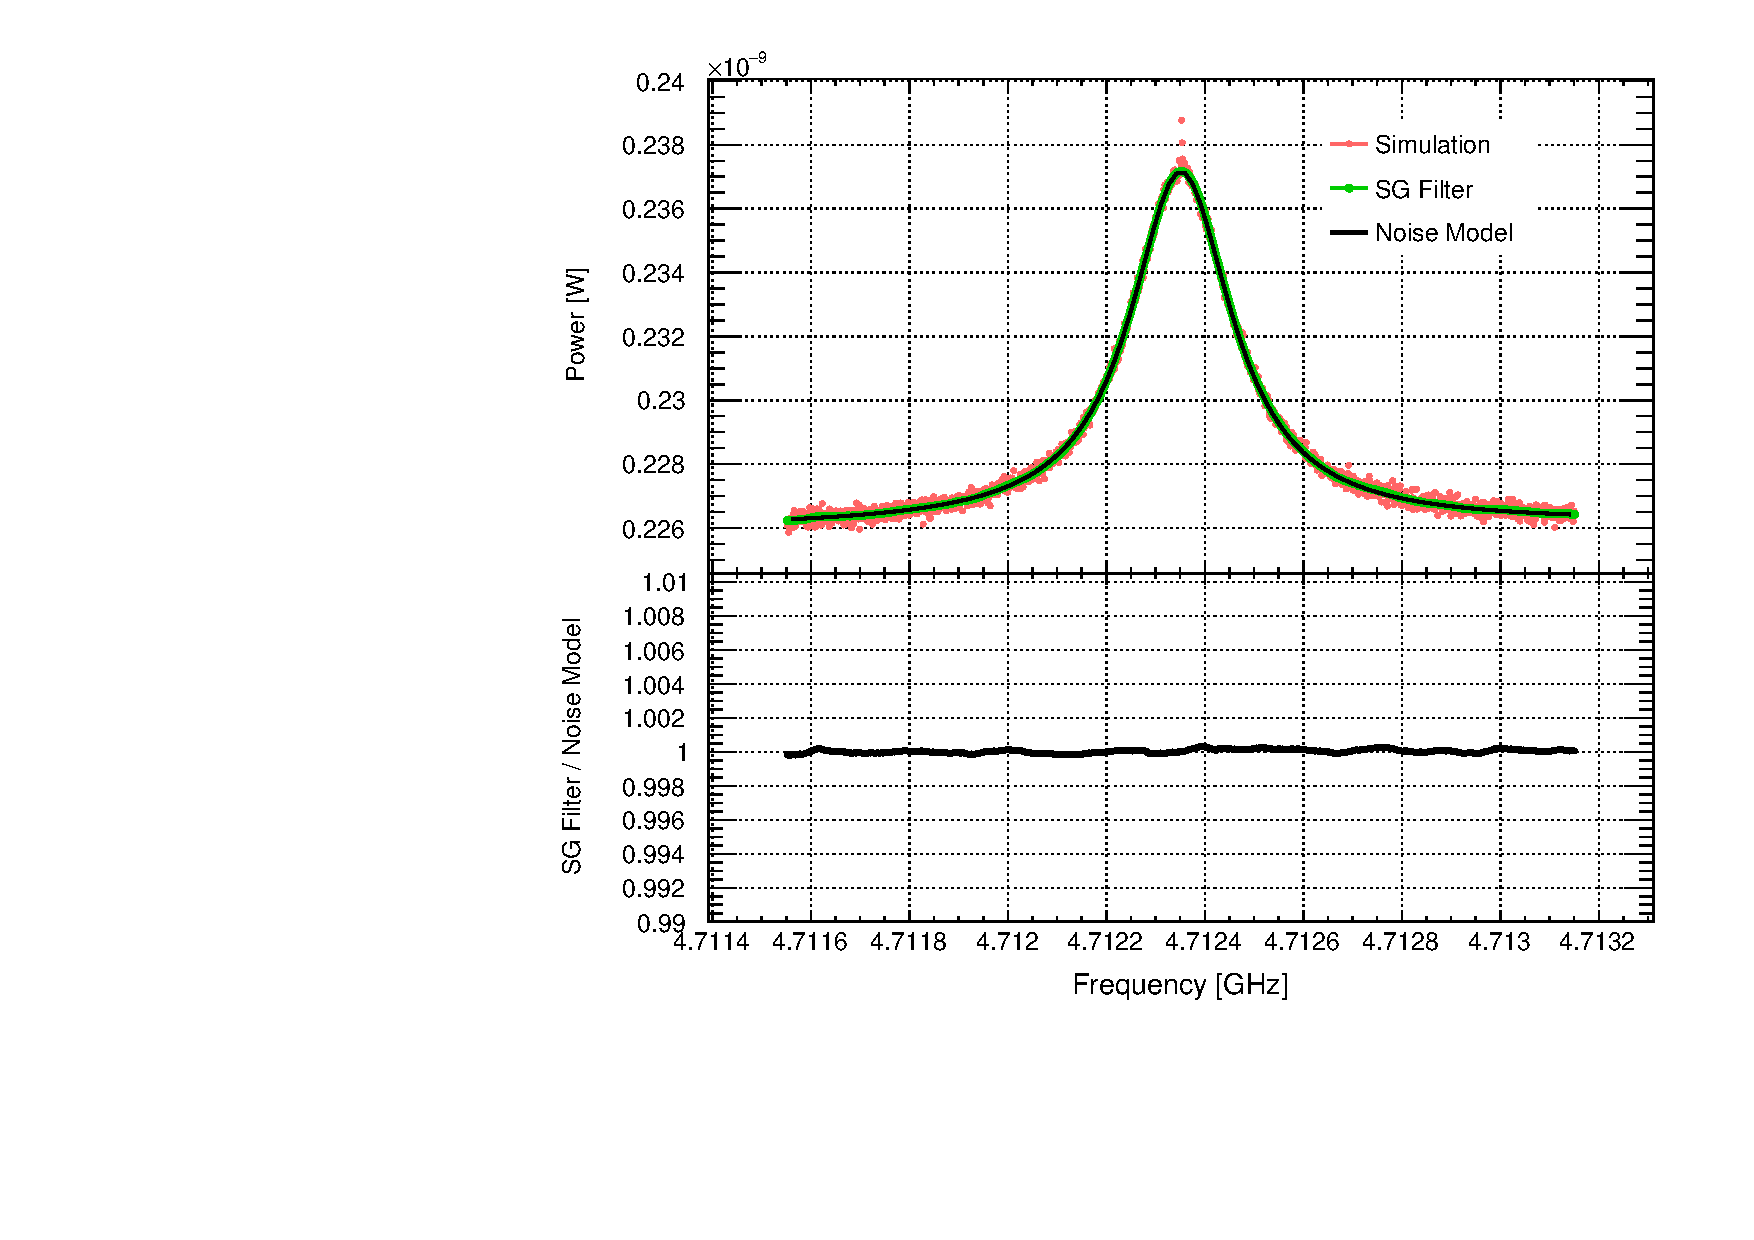
\includegraphics[width=8.6cm]{figures/GeneratedSpectrum_Optimized_SGFilter_NPar_3_Window_141.pdf}
  \caption{Upper panel: 
 The simulated spectrum (red), including the axion signal and the 
noise, is overlaid with the function that models the noise 
${\cal G}_\text{noise}$ (black) and the 
output returned by the SG filter (green). Lower panel: The ratio of the output 
returned by the SG filter to the function ${\cal G}_\text{noise}$.}
  \label{fig:sgcompare}
\end{figure}


\begin{figure} [htbp]
  \centering
%  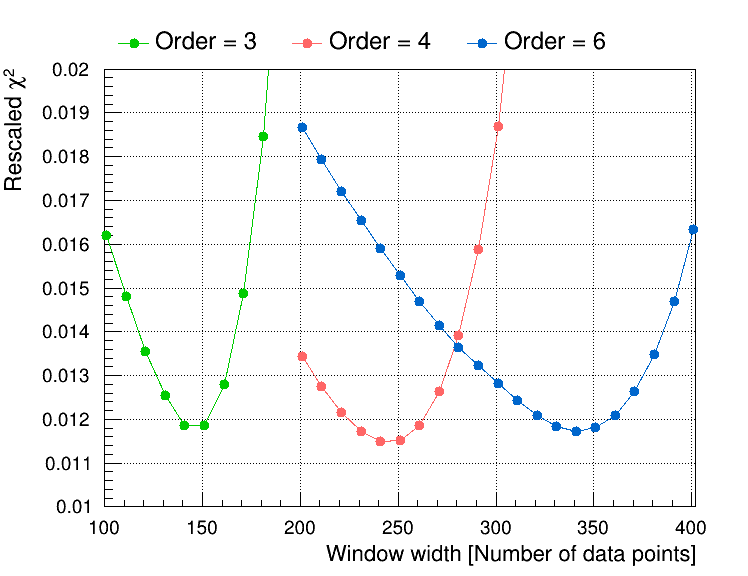
\includegraphics[width=0.4\textwidth,height = 0.25\textwidth]{figures/chi2_Different_Order_Window_SGFilter.png}
  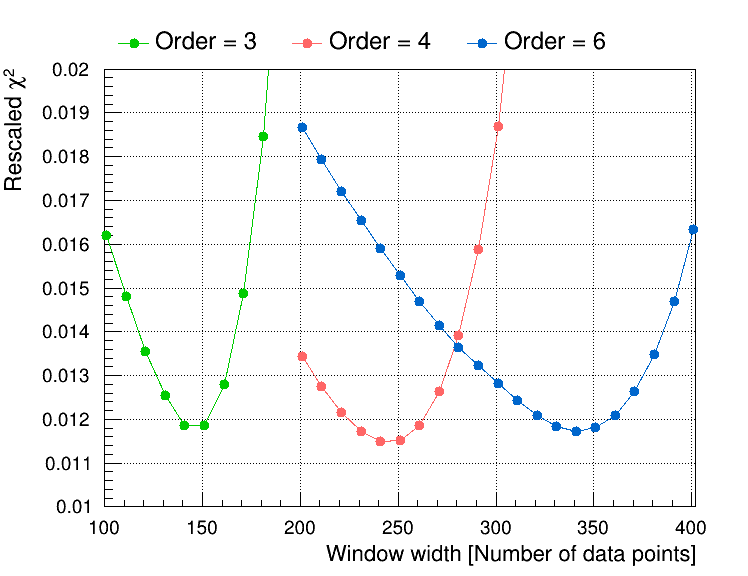
\includegraphics[width=8.6cm]{figures/chi2_Different_Order_Window_SGFilter.png}
  \caption{The difference between the output returned by the SG filter 
  and the function that models the noise spectrum, when various values of 
  window widths and 
  a 3$^\text{rd}$, a 4$^\text{th}$, or a 
  6$^\text{th}$-order polynomial are applied in the SG filter. In this 
  figure, the best choice is a 4$^\text{th}$-order polynomial with 
  a window width of 241 data points (bins). }
  \label{fig:sgoptimize}
\end{figure}
 


\begin{figure} [htbp]
  \centering
  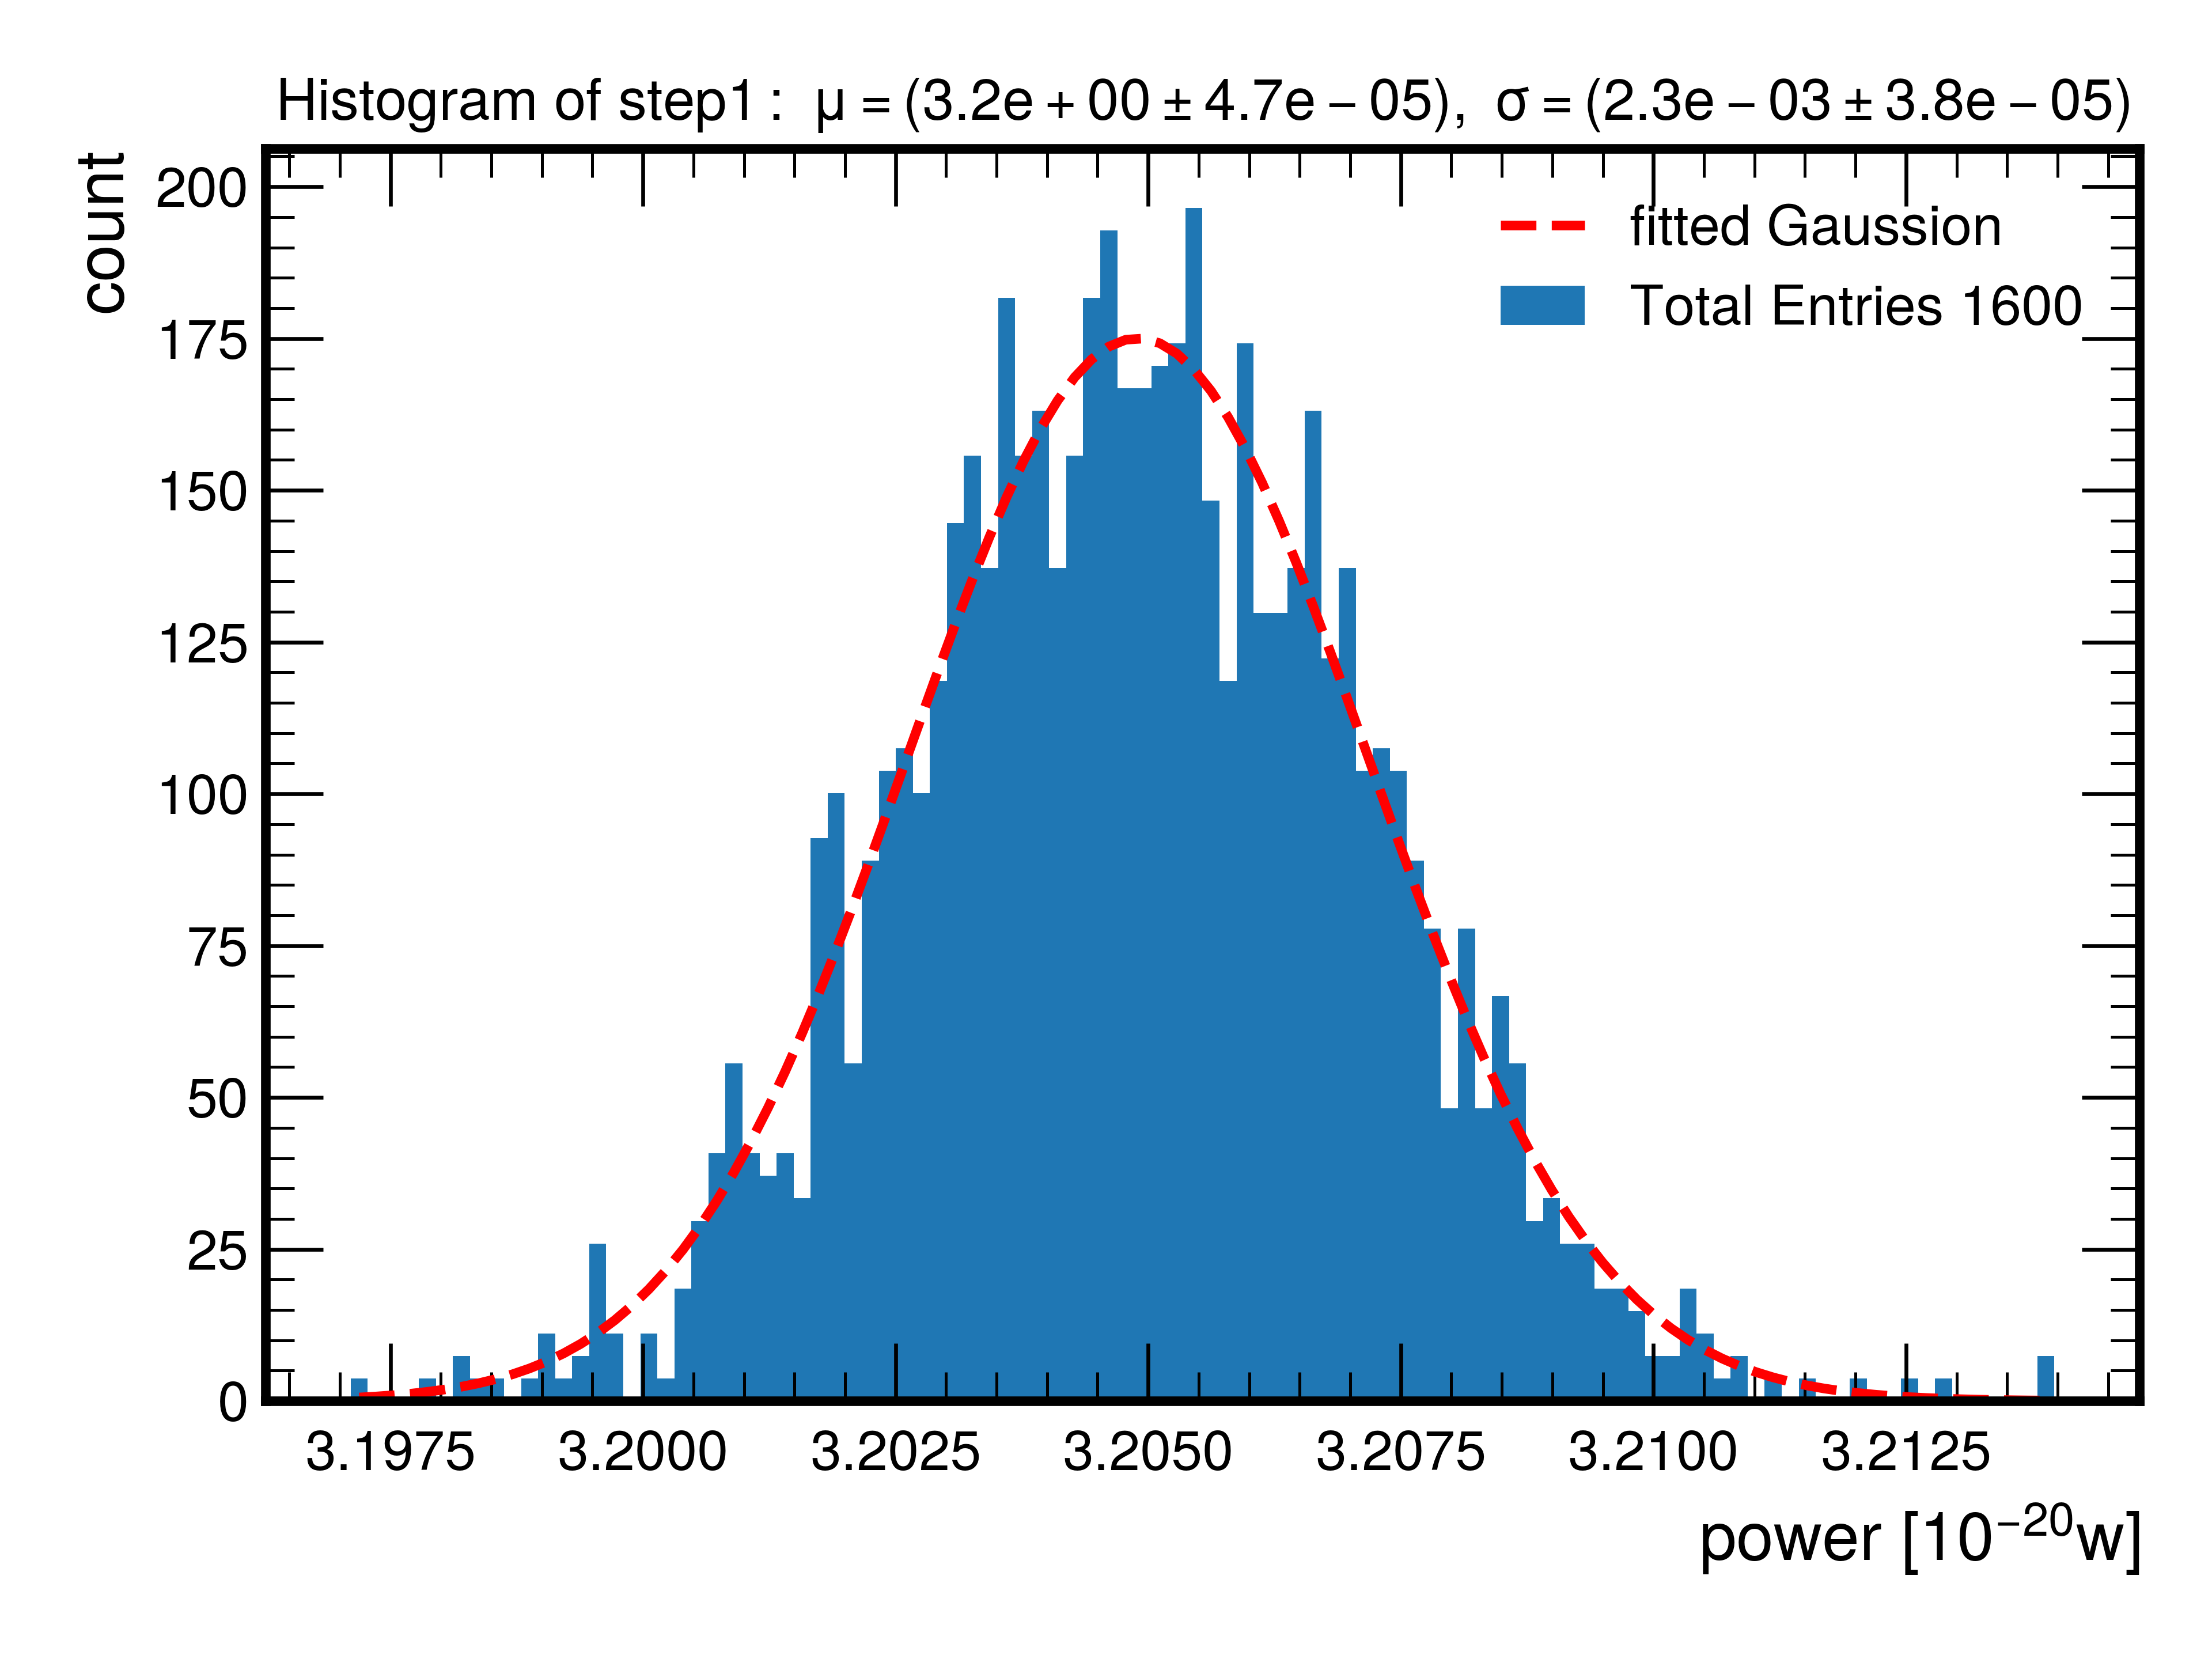
\includegraphics[width=8.6cm]{figures/sysSG_temphistogram.png}
  \caption{An example of the distribution of the measured power after 
applying the SG filter, when 
the cavity resonant frequency is 4.798147~GHz. The distribution contains 
1600 entries and each entry corresponds to the measured power 
in one frequency bin, averaged
over 1920000 subspectra. The mean and the width returned by 
a Gaussian fit to the distribution are used to determine the best choice of 
SG parameters. The fitted Gaussian mean $\mu$ divided by 
$\sqrt{1920000}$ is consistent 
with the fitted Gaussian width $\sigma$. The best choice of SG parameters 
obtained for this scan is a window of 189 data points (bins) with a 
3$^\text{rd}$-order polynomial. 
%The mean $\mu_\text{noise}=3.2\times10^{-20}$~W in 
%a 1-kHz frequency bin would imply a noise temperature of 2.3~K.
}
  \label{fig:noisegauss}
\end{figure}
 

%\begin{figure} [htbp]
%  \centering
%  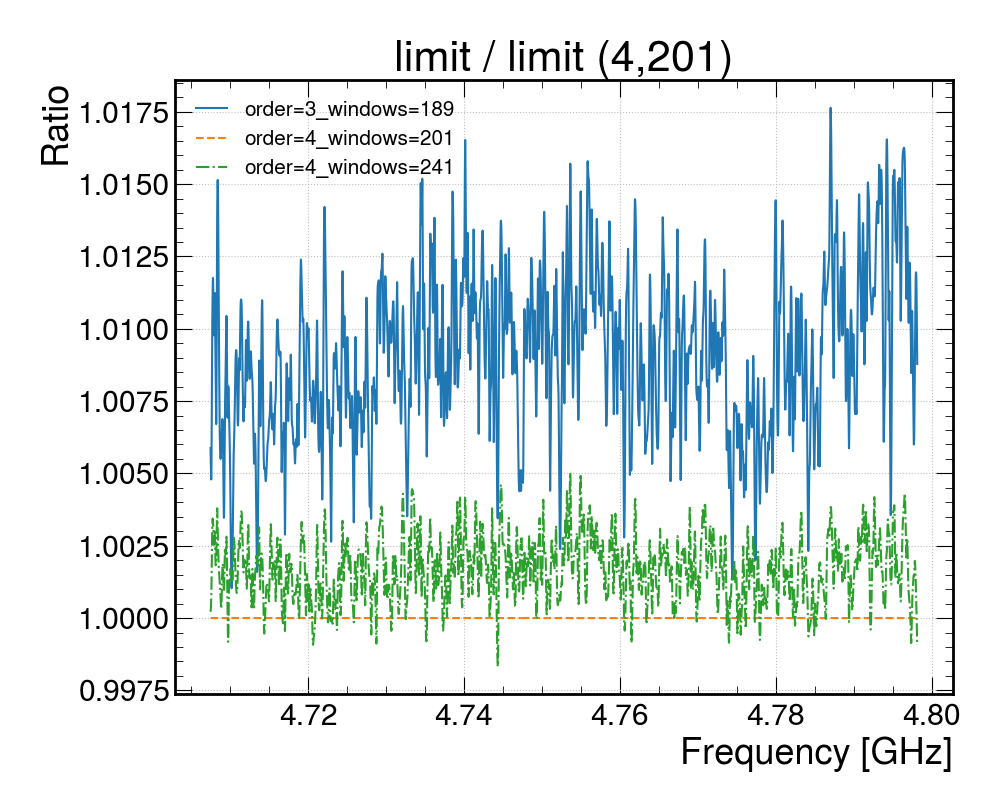
\includegraphics[width=8.6cm]{figures/sys_compareSG_4_201.png}
%  \caption{The ratios of the limits on \gagg\ due to the different choices 
% of the window width and the order of polynomial in the SG filter, with 
%respect to 
% the central results (a window width of 201 bins and the 4$^\text{th}$-order 
% polynomial). The window width of 241 bins and the 4$^\text{th}$-order 
% polynomial are obtained from the optimization after injecting an axion 
%signal on top of a simulated noise spectrum. The window width of 189 bins and 
%the 3$^\text{rd}$-order polynomial are obtained from the optimization 
% after comparing the means and the widths of the measured power distributions.}
%  \label{fig:syssgfilter}
%\end{figure}
 


\section{Results} \label{sec:results}

Figure~\ref{fig:glimit} shows the limits on the axion-two-photon coupling 
\gagg\ and the ratio of the limits on the dimensionless parameter \ggamma\ 
with respect to the KSVZ benchmark value ($\left|g_\text{KSVZ}\right|=0.97$).  
The blue error band indicates the systematic uncertainties as discussed in 
Sec.~\ref{sec:sys}. No limits are placed for the frequency ranges of 
4.710170 -- 4.710190~GHz and 4.747301 -- 4.747380~GHz, which correspond to 
the external signals during the collection of the CD102 data. 
The limits on \gagg\ range from \lolimit\ to \hilimit, with an average 
value of \avelimit; the lowest value comes from the frequency bins with 
additional eight times more data from the rescans, while the highest value 
comes from the frequency bins near the boundaries of the spectrum. 
Figure~\ref{fig:gaggall} displays the \gagg\ limits obtained by TASEH 
together with those from the previous searches. 
The results of TASEH exclude the models with the axion-two-photon
coupling $\gagg\gtrsim \avelimit\GeVinv$, a factor of ten above the benchmark
KSVZ model for the mass range $\mlo < \ma < \mhi \muevcc$ (corresponding to 
the frequency range of $\flo < f_a < \fhi$~GHz). 


The central results shown in Figs.~\ref{fig:glimit}--\ref{fig:gaggall} are 
obtained assuming an axion signal line shape that follows 
Eq.~\eqref{eq:simplesignal}. The analysis that merges bins without 
assuming a signal line shape [$L_{k}=\left.1\middle/5\right.$ 
in Eq.~\eqref{eq:merge_weight}] results in XXXX\% larger values on the 
\gagg\ limits. If a Gaussian signal line shape with an FWHM of 5~kHz is 
assumed instead, the limits will be XXXX than the central results. 



\begin{figure*} [htbp]
  \centering
  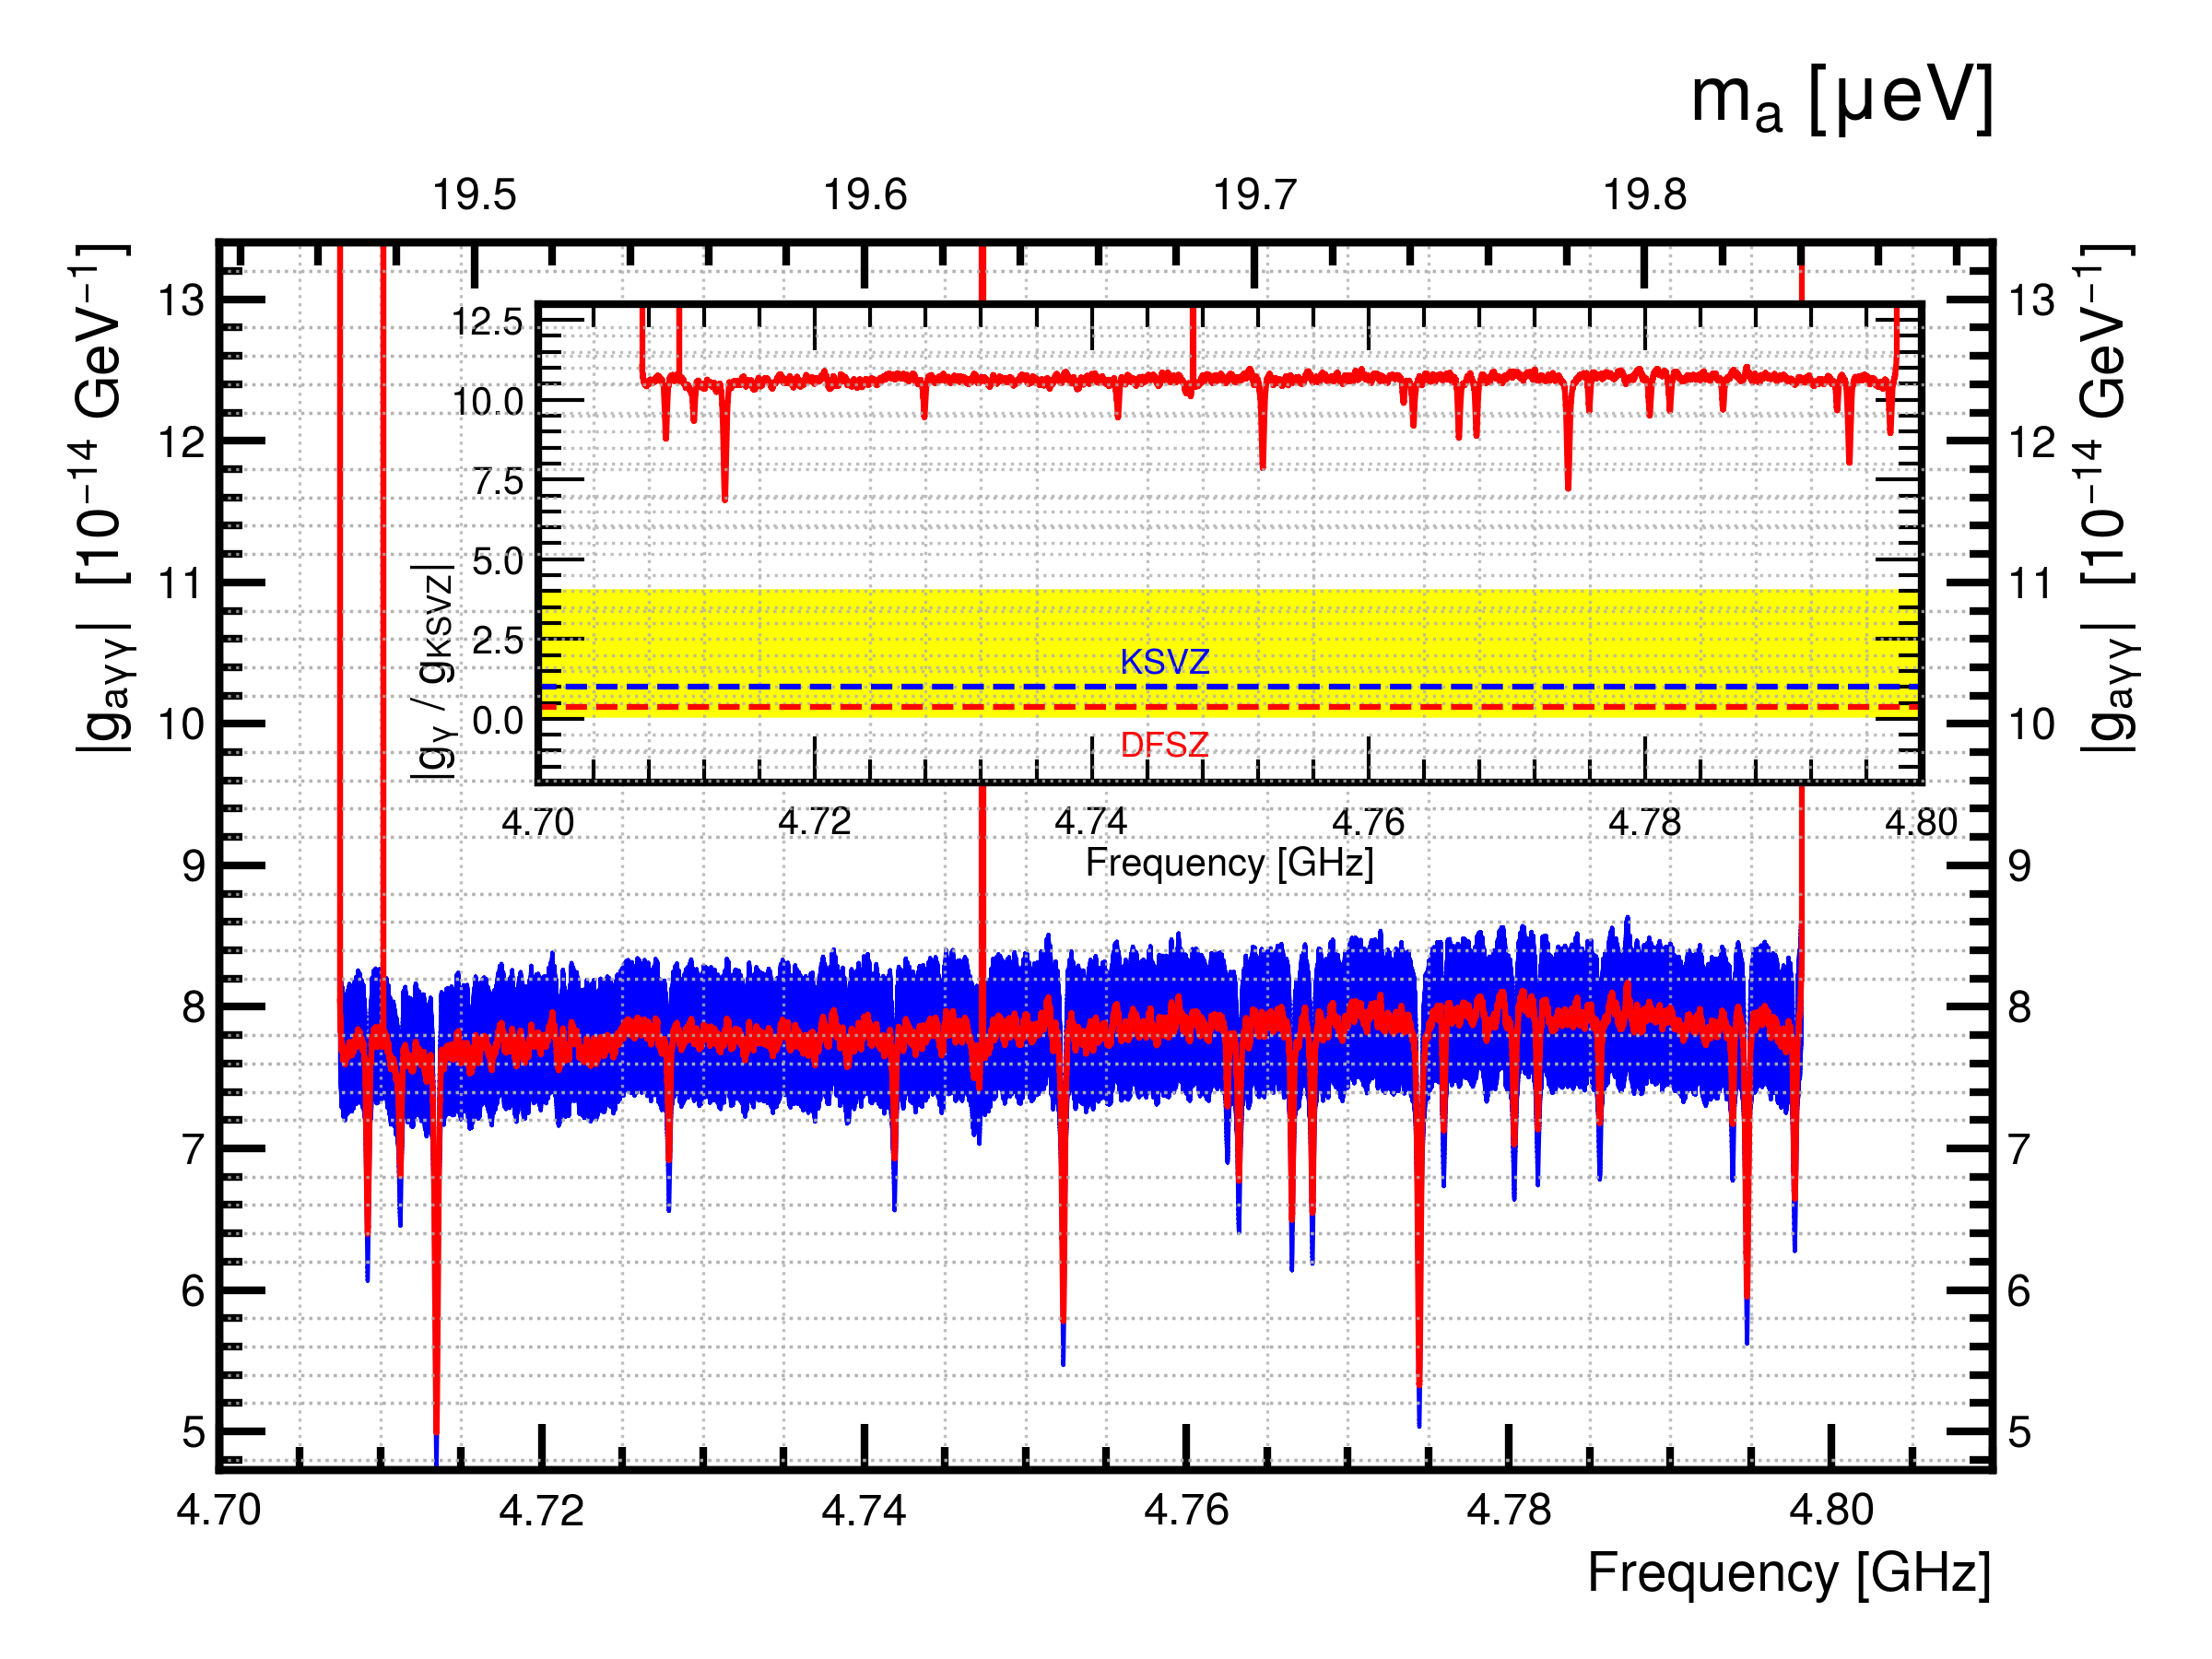
\includegraphics[width=12.9cm]{figures/TASEHonly_limits.png}
%  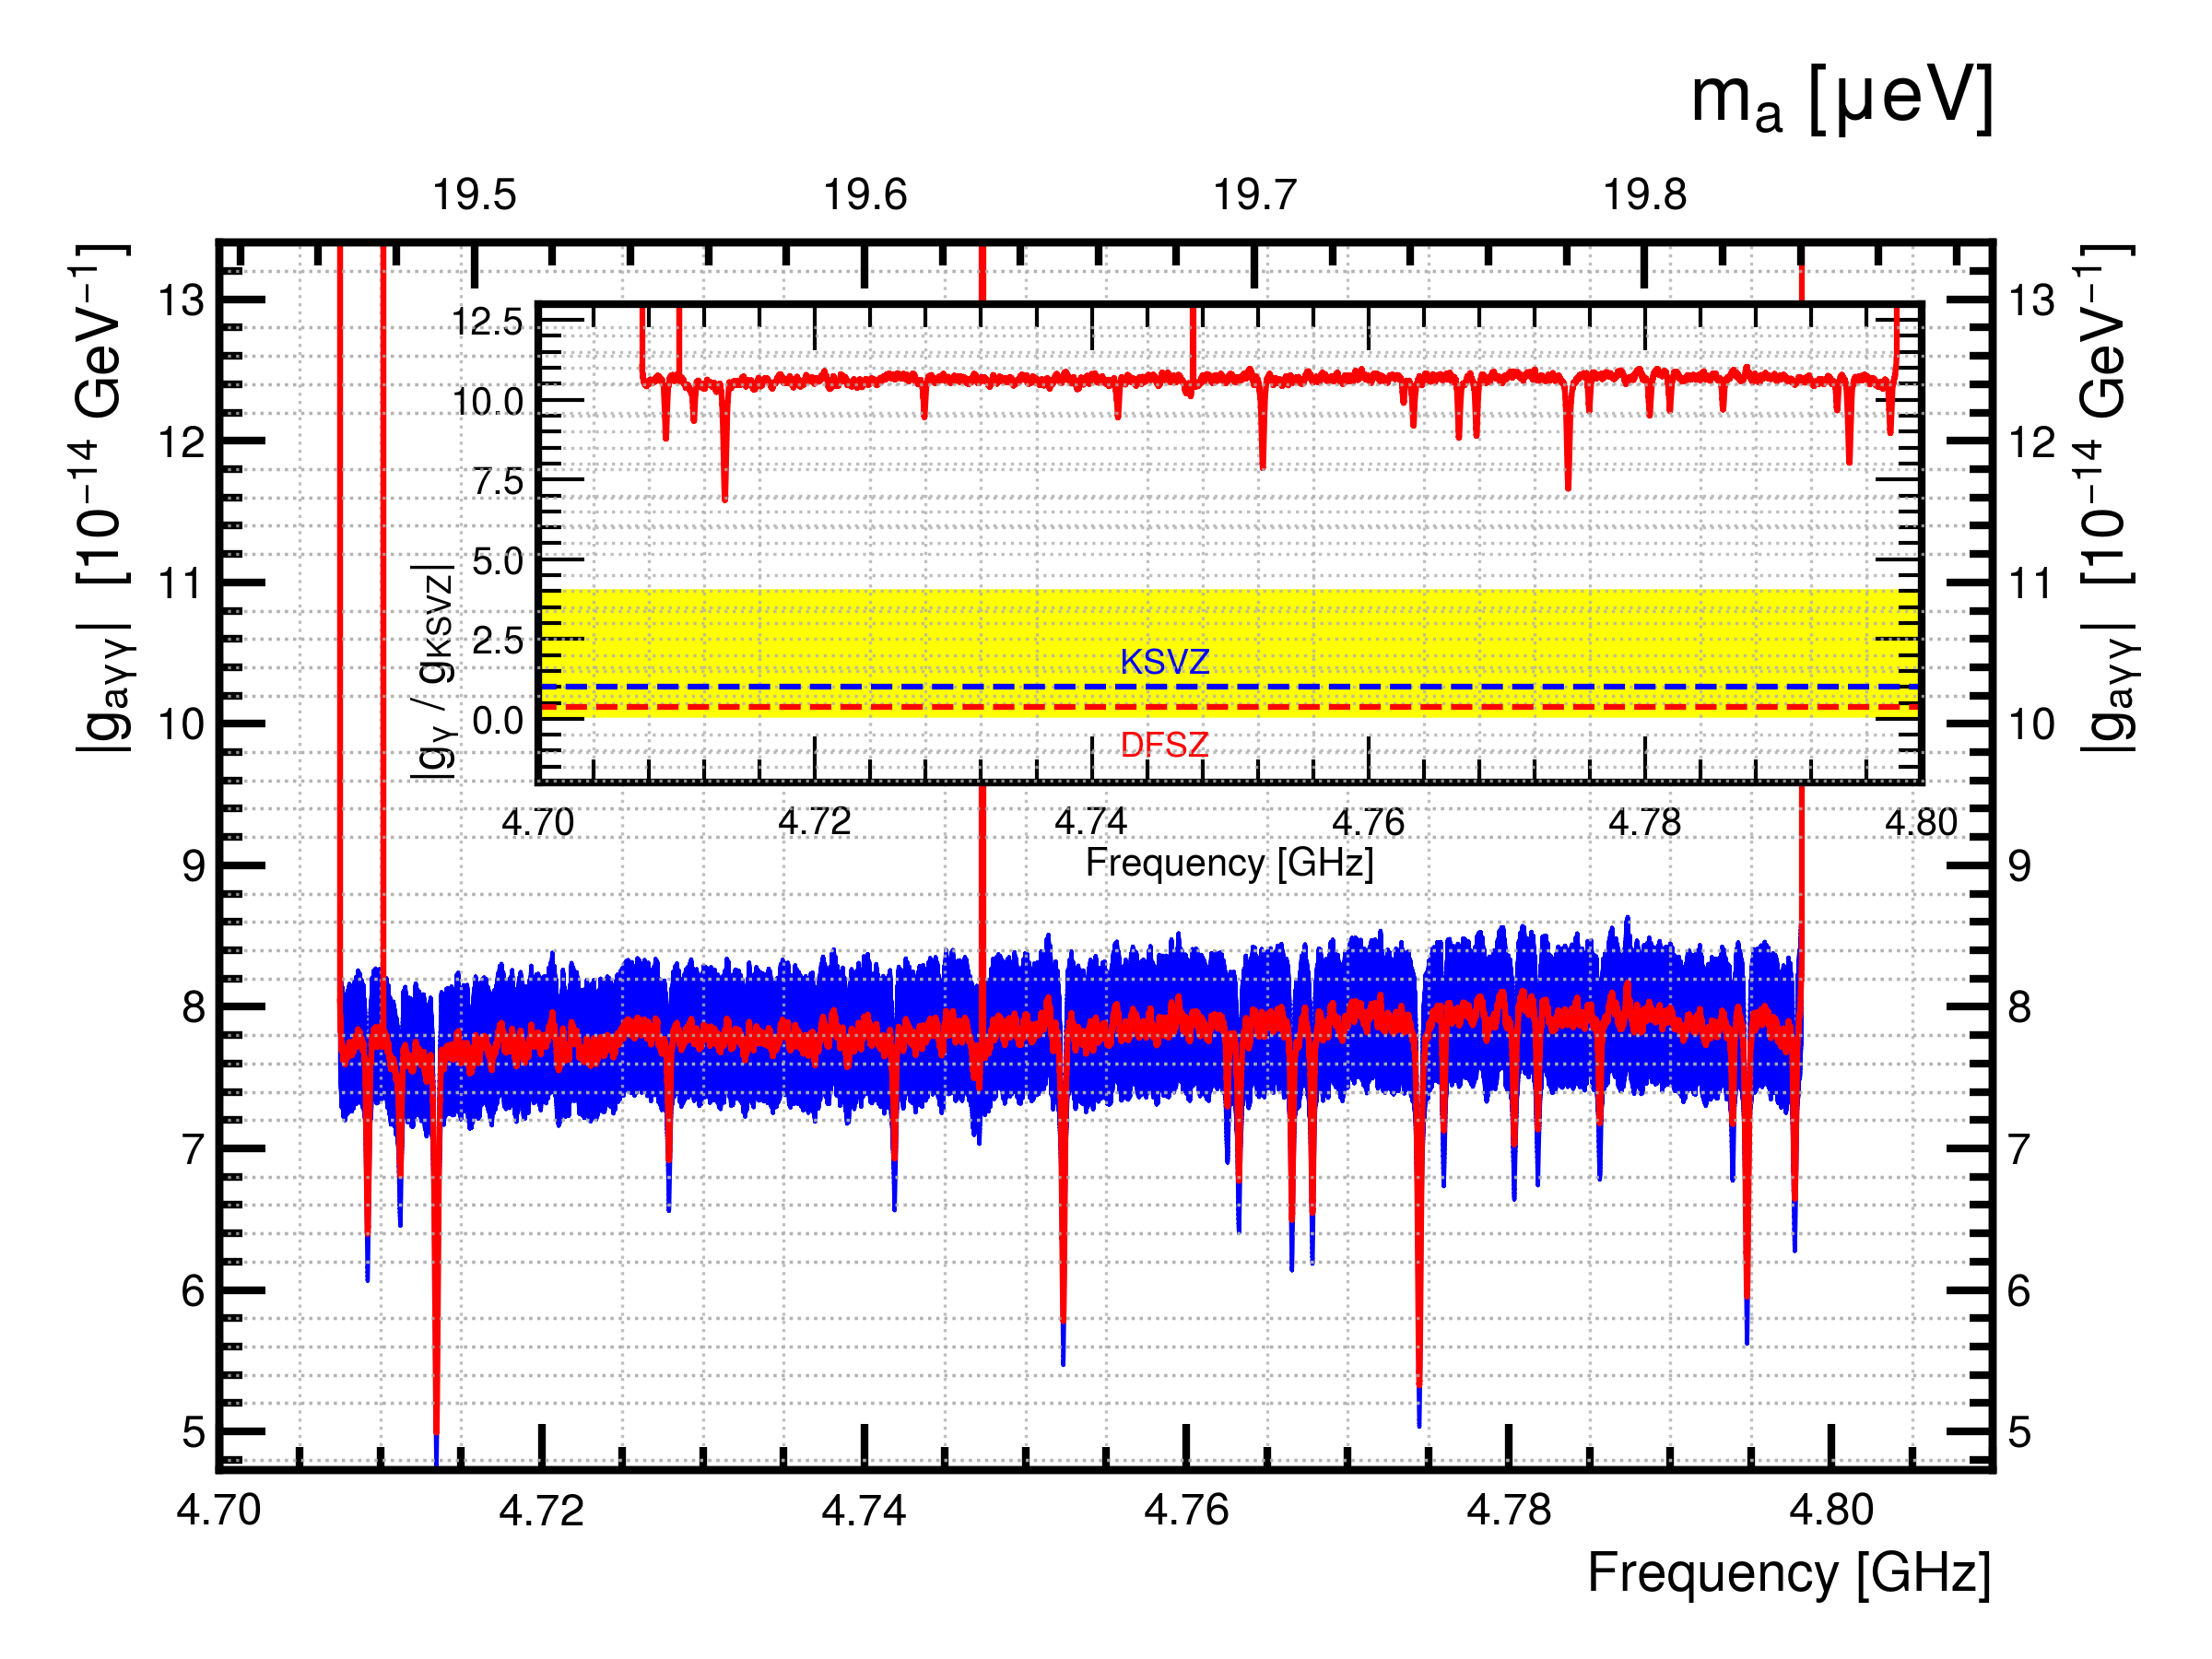
\includegraphics[width=17.2cm]{figures/TASEHonly_limits.png}
%  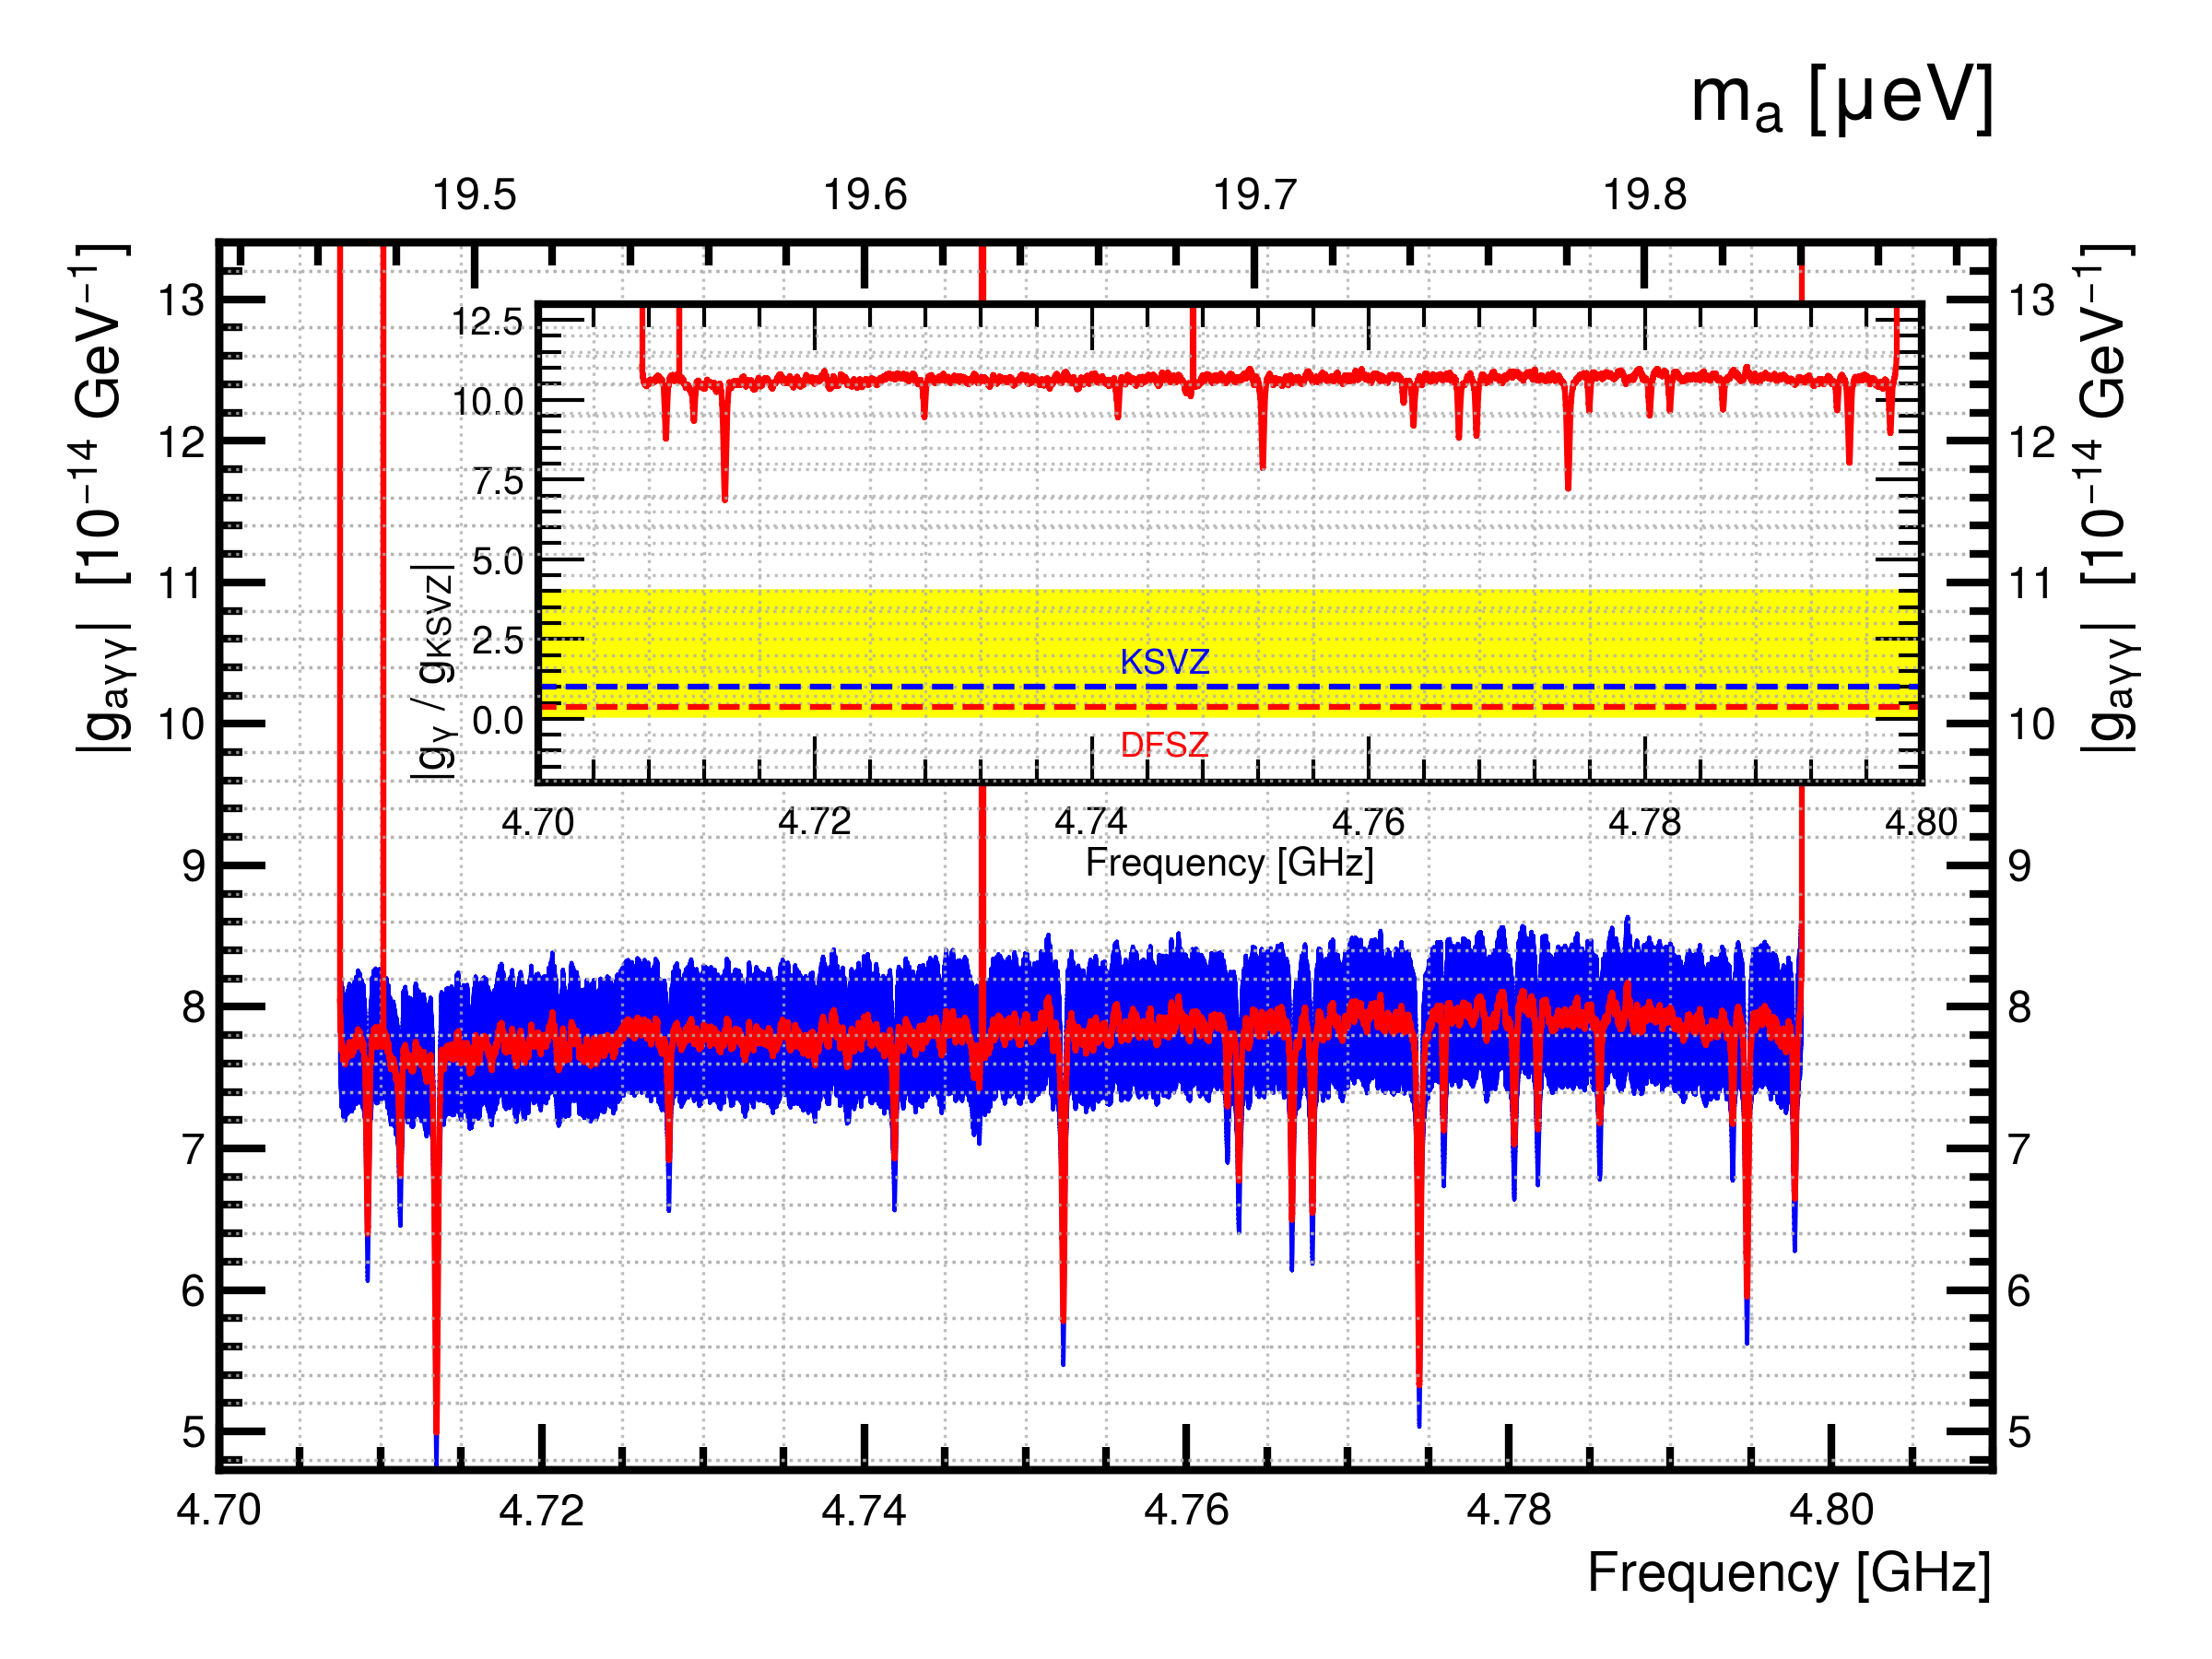
\includegraphics[width=8.6cm]{figures/TASEHonly_limits.png}
  \caption{The limits on \gagg\ and the ratio of the limits on 
\ggamma\ relative to $\left|g_\text{KSVZ}\right|=0.97$ 
  (inset) for the frequency range of 
\flo--\fhi~GHz. The blue error band indicates the systematic 
  uncertainties as discussed in Sec.~\ref{sec:sys}. The yellow 
 band in the inset shows the allowed region of \ggamma\ vs. $m_a$ 
 from various QCD axion models, while the blue and red dashed lines are the 
values predicted by the KSVZ and DFSZ benchmark models, respectively}
  \label{fig:glimit}
\end{figure*}


\begin{figure*} [htbp]
  \centering
 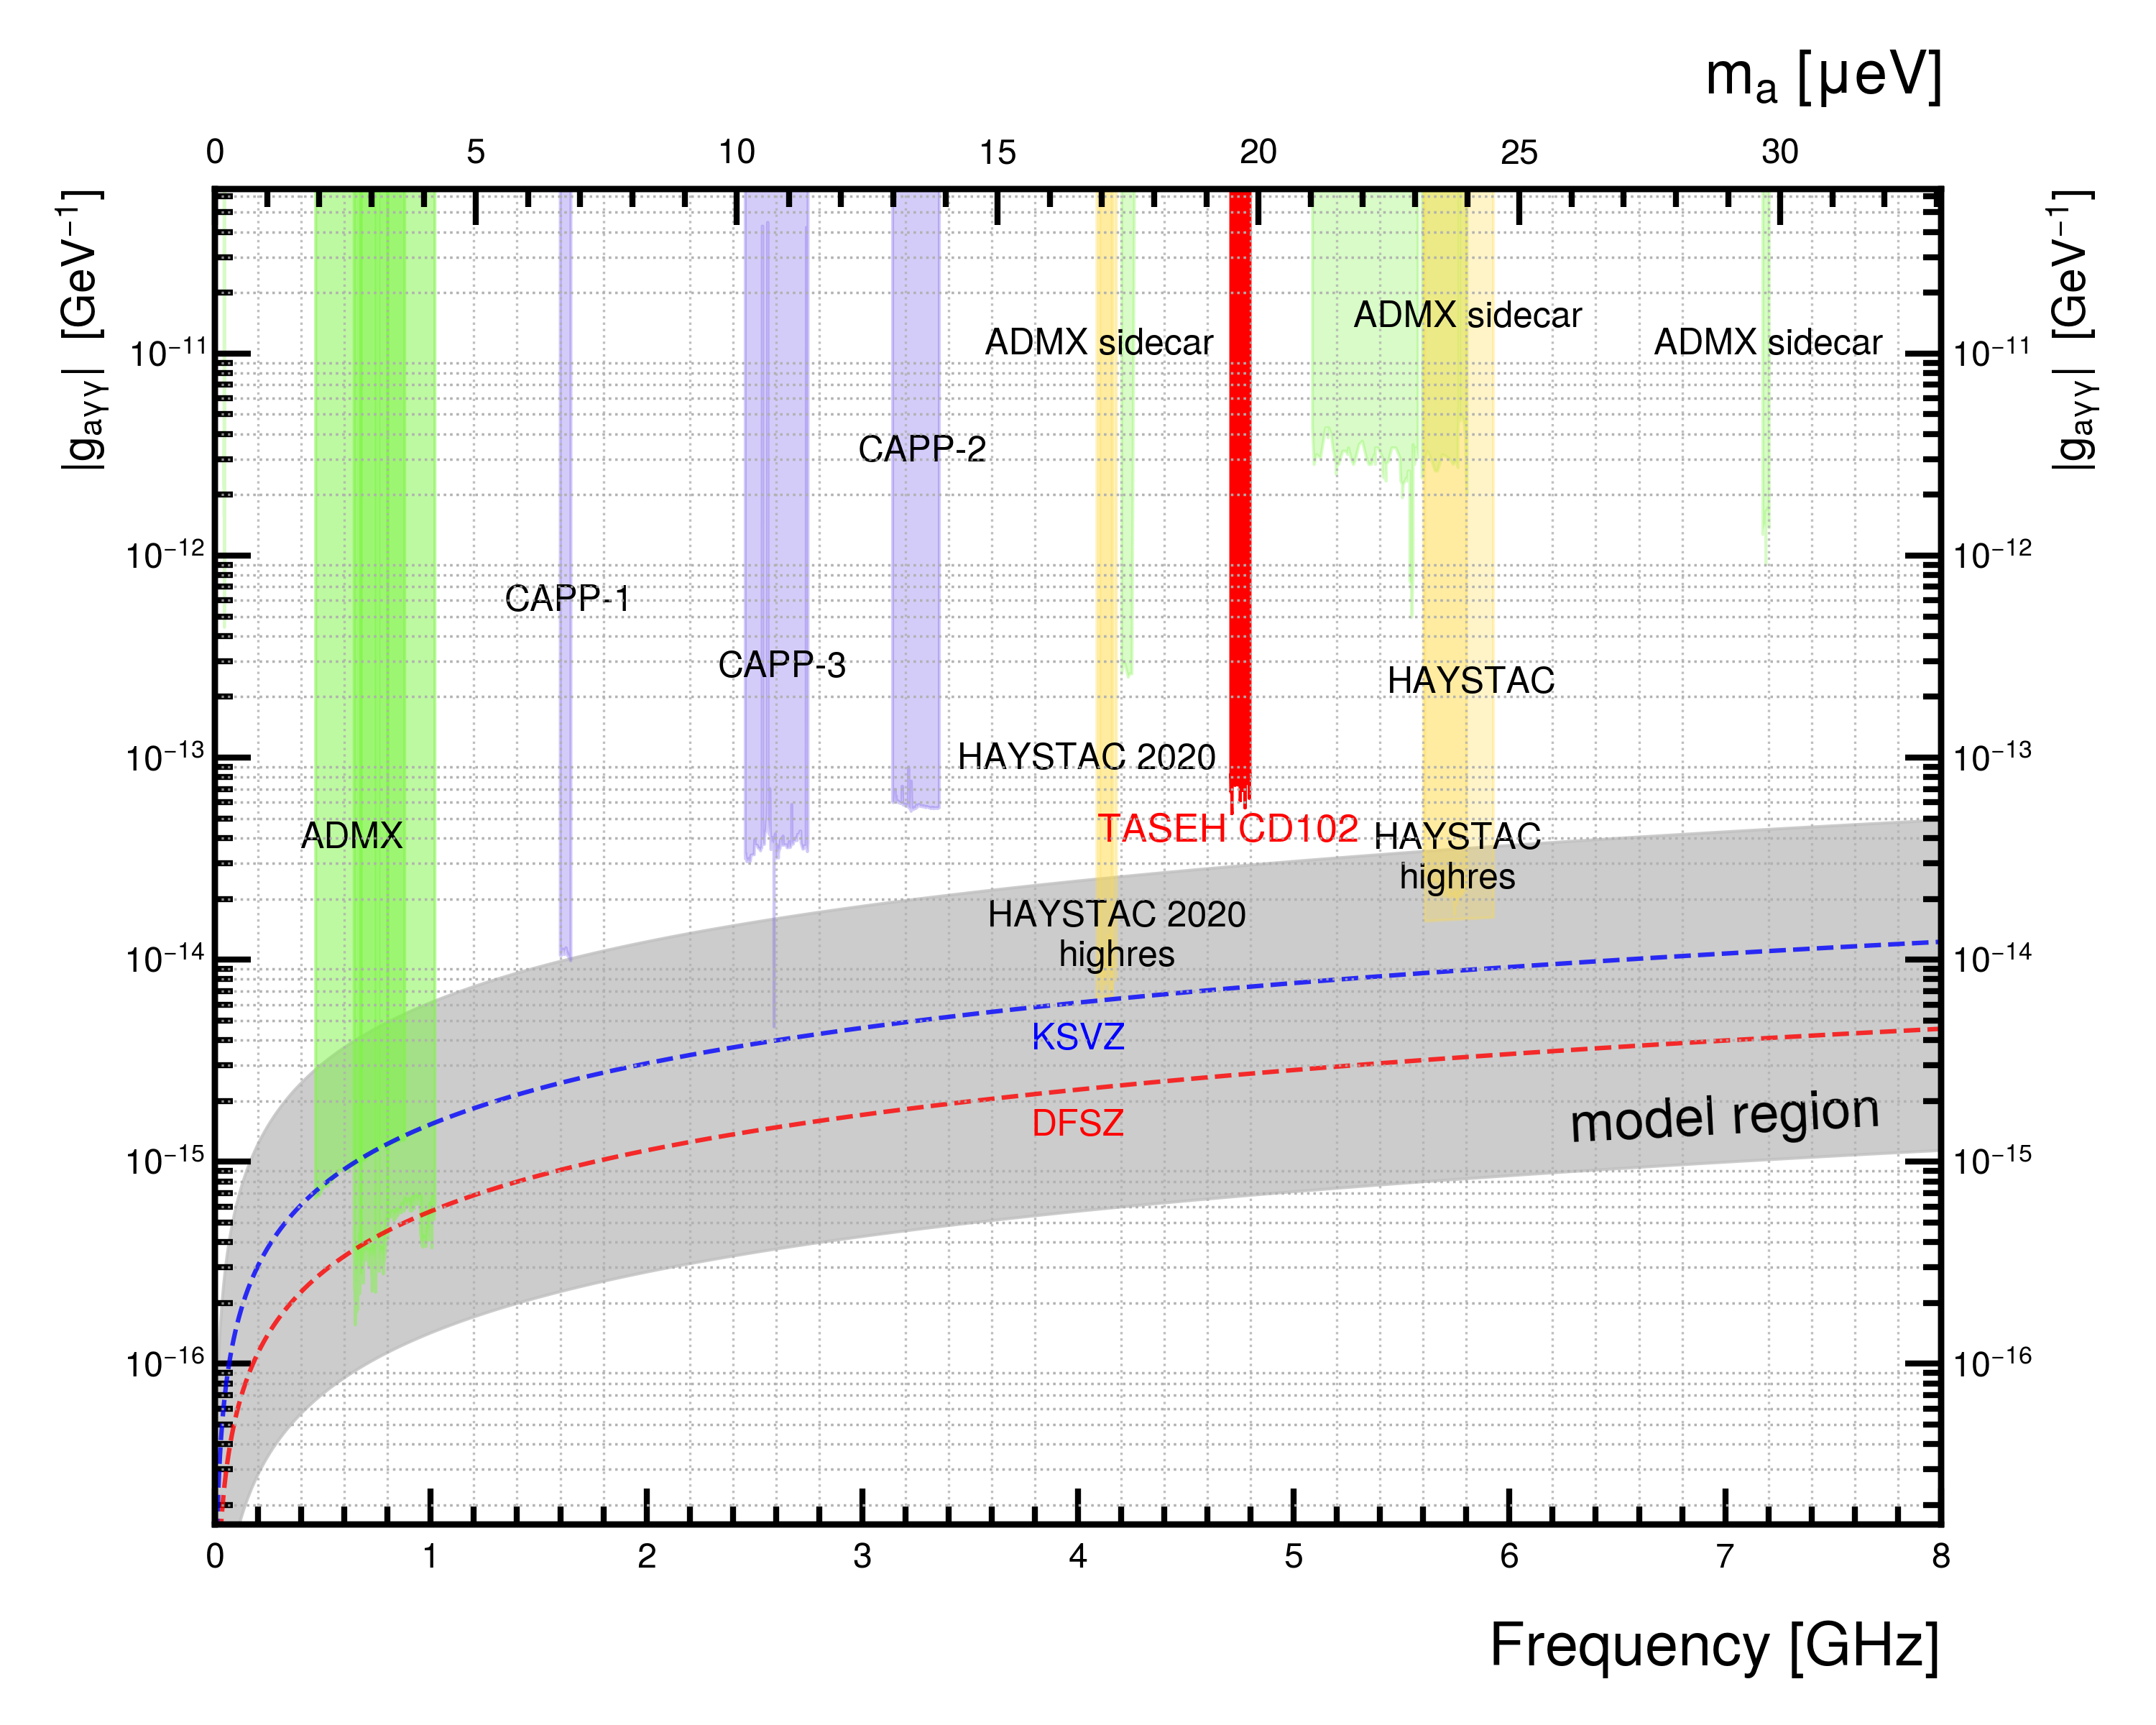
\includegraphics[width=12.9cm]{figures/RealData_limit_allexp.png}
  \caption{The limits on the axion-two-photon coupling \gagg\ for the 
frequency ranges of 0.4--8~GHz, from the CD102 data of TASEH and previous 
searches performed by the ADMX, CAPP, and HAYSTAC Collaborations. The gray 
band indicates the allowed region of \gagg\ vs. $m_a$ from various QCD axion 
models while the blue and red dashed lines are the values predicted by the 
KSVZ and DFSZ benchmark models, respectively.}
  \label{fig:gaggall}
\end{figure*}


%\begin{figure} [htbp]
%  \centering
% 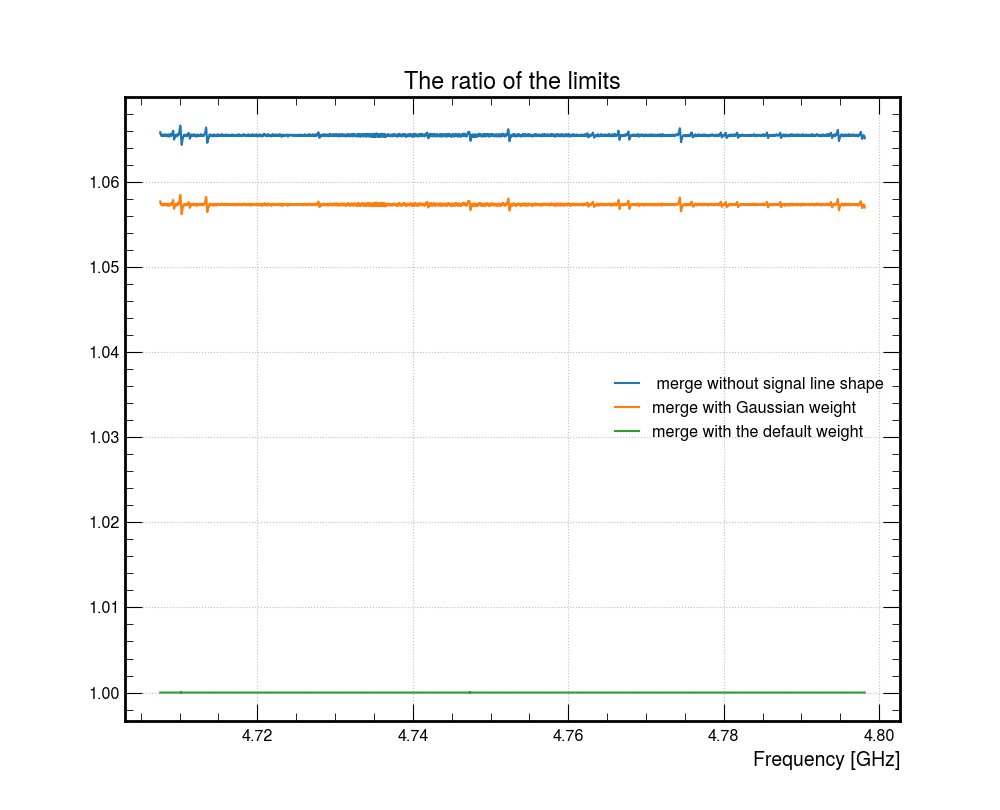
\includegraphics[width=8.6cm]{figures/limitratio_weights.png}
%  \caption{The ratios of the limits on \gagg\ from the merging without 
% assuming a signal line shape (blue) and from the merging with a 
% Gaussian weight (orange), with respect to the central results.}
%  \label{fig:limitratio}
%\end{figure}

%\newpage
\section{Conclusion} \label{sec:conclusion}
This paper presents the analysis details of a search for axions for the mass 
range $\mlo < \ma < \mhi \muevcc$, using the CD102 data collected by the 
Taiwan Axion Search Experiment with Haloscope from October 13, 2021 
to November 15, 2021. 
Apart from the non-axion signals, no candidates with a significance more than
3.355 were found. The synthetic 
axion signals were injected after the collection of data and the 
successful results validate the data acquisition and the analysis procedure. 
The experiment excludes models with the 
axion-two-photon coupling $\gagg\gtrsim \avelimit\GeVinv$ at 95\% C.L.,
 a factor of eleven 
above the benchmark KSVZ model. The sensitivity on \gagg\ reached by TASEH 
is three orders of magnitude better than the existing limits. 
It is also the first time that a haloscope-type experiment places 
constraints in this mass region. The readers shall be aware that haloscope 
experiments assume 
that 100\% of the dark matter is the axion. In addition, the local dark 
matter density, which is used to compute the expected axion signal power, 
can have an uncertainty as large as 50\%; this uncertainty 
is typically considered an external 
uncertainty and not included in the experimental results. 

The target of TASEH is to search for axions for the mass range of 
16.5--20.7\muevcc\ corresponding to a frequency range of 4--5~GHz, with a 
capability to be extended to 2.5--6~GHz in the future. 
In the coming years, several upgrades are expected, including: the use of a 
quantum-limited Josephson parametric amplifier as the first-stage amplifier, 
the replacement of the existing dilution refrigerator with a new one that has 
a magnetic field of about 9~Tesla and a larger bore size, and the development 
of a new cavity with a significantly larger effective volume. %These upgrades 
%will reduce the added noise by a factor of 10 and increase the magnetic 
%field and the cavity volume by a factor of 1.125 and 5, respectively. 
With the improvements of the experimental setup and several years of data 
taking, TASEH is expected to probe the QCD axion band in the target mass range.




\begin{acknowledgments}
We thank Chao-Lin Kuo for his help to initiate this project as well as 
discussions on the microwave cavity design, Gray Rybka and Nicole Crisosto 
for their introduction of the ADMX experimental 
setup and analysis, Anson Hook for the discussions and the review of the 
axion theory, and Jiunn-Wei Chen, Cheng-Wei Chiang, Cheng-Pang Liu, and 
Asuka Ito for the discussions of future improvements in axion searches.  
  The work of the TASEH Collaboration was funded by 
the Ministry of Science and Technology (MoST) of Taiwan with grant numbers 
MoST-109-2123-M-001-002, MoST-110-2123-M-001-006, MoST-110-2112-M-213-018, 
MoST-110-2628-M-008-003-MY3, 
and MoST-109-2112-M-008-013-MY3, and by the Institute of Physics, Academia 
Sinica. 

\end{acknowledgments}

\appendix
%\newpage
\section{Derivation of the Function that Models the Noise Spectrum} 
\label{sec:cavitynoise}

The background noise from a cavity is governed by the thermal noise and the 
vacuum fluctuation. %from the cavity. 
According to Planck's law in one dimension (1D), the spectral density of 
the electromagnetic noise from the cavity, thermalized with an environment of 
temperature $T_{\rm c}$, through a transmission line is 
\begin{equation}
\label{eq:cavity_thermal_spectral_density}
    S(\omega) = \hbar\omega \left( \frac{1}{e^{\hbar\omega/k_{\rm B}T_{\rm c}} - 1} +\frac{1}{2} \right),
\end{equation}
where $\omega$ is the angular frequency, $\hbar$ is the reduced Planck's 
constant, and $k_{\rm B}$ is the Boltzmann constant. 
%The first and the second 
%terms in Eq.~\eqref{eq:cavity_thermal_spectral_density} are the thermal noise 
%and the vacuum fluctuation from the cavity, respectively. The spectrum is 
%white when considering a narrow frequency span.

However, the cavity body (the materials that form the cavity itself) may not 
be thermalized with its 1D electromagnetic environment. To understand the 
noise spectrum from the cavity near its 
resonant frequency $\omega_{\rm c}/2\pi$ in this scenario, the model in 
Fig.~\ref{fig:cavity_in_out} is considered. Through a probe the cavity field 
mode $c$ is coupled to the modes $a_2$ of a 1D transmission line, representing
 the path toward a signal receiver, with a rate $\kappa_2$. The cavity field 
is also coupled to the modes of the cavity body $a_0$, representing the 
intrinsic loss, with a rate $\kappa_0$. In a steady state, 
the quantum input-output theory leads to a relation between the outgoing field 
from the cavity to the 1D transmission line, $a_{\rm 2,out}$, and the incoming
 fields, $a_{\rm 2,in}$ and $a_{\rm 0,in}$, through the elements of the 
cavity scattering matrix:
\begin{equation} \label{eq:outgoing_field}
	 a_{\rm 2,out} = S^{*}_{\rm 22} a_{\rm 2,in} + S^{*}_{\rm 20} a_{\rm 0,in},
\end{equation}
where $S_{\rm 22} = \frac {\kappa_0 - \kappa_{\rm 2} + i 2 \Delta} {\kappa_0+\kappa_{\rm 2} + i 2 \Delta}$, $S_{\rm 20} = \frac {2\sqrt{\kappa_0 \kappa_{\rm 2}}} {\kappa_0+\kappa_{\rm 2} + i 2 \Delta}$,
and $\Delta = \omega-\omega_{\rm c}$ is the detuning. 

As both incoming fields are in a thermal state, $\langle a_{i,\rm in}(0) a_{i,\rm in}(\tau) \rangle = n_{\rm th}(T_i) \delta(\tau)$, where $n_{\rm th}(T_i) = \frac{1}{e^{\hbar\omega/k_{\rm B}T_i} - 1}$ is the mean thermal photon number 
of the incoming field $a_{i,\rm in}$ at the temperature $T_i$, and 
$\delta(\tau)$ is the $\delta$-function. In the model the incoming field 
$a_{\rm 2,in}$ comes from a nearby attenuator, anchored to the mixing flange, 
in the transmission line 
with a temperature $T_{\text mx} \equiv T_{\rm 2}$, and $a_{\rm 0,in}$ comes 
from the cavity body with a temperature $T_{\text c} \equiv T_{\rm 0}$.

By defining the effective temperature $\Tilde{T}_i = \left( n_{\rm th}(T_i) + \frac{1}{2} \right) \hbar\omega/k_{\rm B}$,
the power spectral density of the outgoing field of the transmission line 
modes is
\begin{equation}
\label{eq:spectrum_relation}
\begin{aligned}
    S_{\rm out}(\omega) 
    =& \int_{-\infty}^{\infty} \hbar\omega \left(\langle a_{2,\rm out}(0) a_{2,\rm out}(\tau) \rangle + \frac{1}{2} \right) e^{-i\omega\tau} d\tau \\
    =& |S_{\rm 22}|^2 k_{\rm B} \Tilde{T}_2 + |S_{\rm 20}|^2 k_{\rm B} \Tilde{T}_0.
\end{aligned}
\end{equation}
%The total output noise can be viewed as the sum of the reflection of the 
%incoming noise from the attenuator by the cavity and the transmission of the 
%noise from the cavity body through the cavity. 
The total output noise can be viewed as the sum of the reflection of the 
incoming noise from the attenuator and the transmission of the noise from the 
cavity body itself.
Via the unitary property of 
the cavity scattering matrix, i.e. $|S_{\rm 22}|^2+|S_{\rm 20}|^2=1$,
\begin{equation}
\label{eq:spectrum_relation_Lorentz}
\begin{aligned}
    S_{\rm out}(\omega) =  k_{\rm B} \Tilde{T}_2 + k_{\rm B} (\Tilde{T}_0 - \Tilde{T}_2) L(\omega),
\end{aligned}
\end{equation}
where $L(\omega) = |S_{\rm 20}|^2 = \frac {\kappa_0 \kappa_{\rm 2}}  {(\kappa_0+\kappa_{\rm 2})^2/4 + \Delta^2}$ is a Lorentzian function with a FWHM 
$\kappa_0+\kappa_{\rm 2}$. Therefore, the noise spectrum has a flat background
 determined by the incoming noise of the attenuator with an effective 
temperature $\Tilde{T}_{\rm 2}$, plus an excess Lorentzian peak centered at 
$\omega_{\rm c}$ determined by the effective temperature difference 
$\Tilde{T}_{\rm 0} - \Tilde{T}_{\rm 2}$. (The center Lorentzian structure 
can even be a dip if ${T}_{\rm 0} < {T}_{\rm 2}$.)

\begin{figure}[htbp]
    \centering
    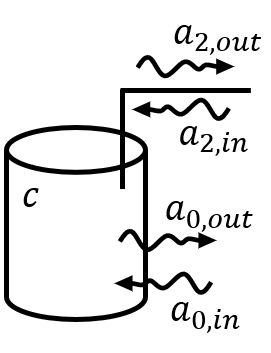
\includegraphics[width=8.6cm]{figures/inout.png}
    \caption{A cavity is coupled to the modes of transmission line $a_2$ with 
the rate $\kappa_2$ and the modes of the cavity body $a_0$ with the rate 
$\kappa_0$.}
    \label{fig:cavity_in_out}
\end{figure}





%\section{Appendixes}
\bibliographystyle{apsrev4-2}
\bibliography{main}% Produces the bibliography via BibTeX.

\end{document}
%
% ****** End of file apssamp.tex ******
